\documentclass{report}
\usepackage{fontspec}

\newfontfamily\aplfont[Scale=0.90]{APL385.ttf}
\setmonofont[Scale=0.90]{APL385.ttf}

\usepackage{threeparttable}
\usepackage{soul}
\usepackage{pifont}
\usepackage{dirtytalk}
\usepackage{graphicx}
\usepackage{glossaries}
\usepackage{listings}
\usepackage{threeparttable}
\usepackage{todonotes}
\usepackage{soul}
\usepackage{amsmath,amssymb}
\usepackage{caption}
\usepackage{url}
\newcommand{\source}[1]{\caption*{Source: {#1}} }
\newcommand{\cmark}{\ding{51}}
\usepackage[absolute]{textpos}

\usepackage[style=ieee]{biblatex}
\usepackage{listings}
\addbibresource{main.bib}

\newacronym{APL}{APL}{A Programming Language}
\newacronym{GPU}{GPU}{graphics processing unit}
\newacronym{SIMD}{SIMD}{single-instructor multiple-data}
\newacronym{API}{API}{application programming interface}
\newacronym{IR}{IR}{intermediate representation}
\newacronym{GPGPU}{GPGPU}{general purpose computing on GPUs}
\newacronym{NFV}{NFV}{network function virtualization}
\newacronym{LTL}{LTL}{linear temporal logic}
\newacronym{IDE}{IDE}{integrated development environment}

\lstdefinestyle{mystyle}{
    % basicstyle=\aplfont\footnotesize,
    breaklines=true,
    numbers=left,
    numbersep=3pt,
}
\lstset{style=mystyle}

\usepackage{titling}
\renewcommand\maketitlehooka{\null\mbox{}\vfill}
\renewcommand\maketitlehookd{\vfill\null}

\makeatletter
\newcommand{\quickwordcount}[1]{%
  \immediate\write18{texcount -1 -sum -merge #1.tex > #1-words}%
  \immediate\openin\somefile=#1-words%
  \read\somefile to \@@localdummy%
  \immediate\closein\somefile%
  \setcounter{wordcounter}{\@@localdummy}%
  \@@localdummy%
}
\makeatother

\begin{document}

\begin{titlepage}
    $ $ % very important line do not remove
    \vspace{4cm}
    \begin{center}
        \huge{Static Semantics of Rank Polymorphism}
    \end{center}

    \begin{figure*}[ht]
        \centering
        \begin{minipage}[b]{0.35\textwidth}
            
\includegraphics[width=\textwidth]{./assets/01-standard-vertical-black-text.png}
        \end{minipage}
    \end{figure*}

    \begin{textblock}{200}(10,12)%
    \obeylines
    \setlength{\parskip}{0cm}
        University of St Andrews
        Master of Computer Science - DEPEND
        Master's Thesis
        Juuso Haavisto
        Supervisor: \textit{Dr.} Christopher Brown
        June 2021
    \end{textblock}%

\end{titlepage}

\section*{Declaration}

I declare that this material, which I now submit for assessment on the program of study leading to the award of Master of Science in Dependable Software Systems, is entirely my own work and has not been taken from the work of the others save and to the extent that such work has been cited and acknowledged within the text of my work. This work was performed during the current academic year except where otherwise stated. The main text of this project report consists of \quickwordcount{main} words. In submitting this project to the University of St Andrews, I give permission for it to be made available for use in accordance with the regulations of the University Library. I also give permission for the report to be made available on the Web, for this work to be used in research within the University of St Andrews, and for any software to be released on an open-source basis. I retain the copyright in this work and ownership of any resulting intellectual property.

\section*{Acknowledgements}

I thank my supervisor Christopher Brown for helping me to learn Idris.

\begin{abstract}

% Purpose
The prevalence of multi-core systems in the 21st century has increased interest in programming languages for parallel computation. In general, the challenge of parallel computation can be considered two-fold: 1) to have a language that can express and promote parallel constructs and 2) that such language allows static inference of parallel patterns to schedule the work on hardware efficiently. This study focuses on the second part, proposing static semantics using dependent types for an array programming language that exhibits rank polymorphism. We conduct our research empirically using the Idris language for dependent types and target a three-rank fragment of APL as the modeled parallel language. Our work can be considered an enhancement effort of introducing static type checking to APL using Idris. We demonstrate how rank polymorphism can be captured for scalars, vectors, and matrices using a generic one-dimensional vector with stride information. We also demonstrate how dependent types can statically capture so-called shape errors, lacking in current-day APL implementations. Further, we stipulate how Idris can statically type compute kernels for parallel execution on graphics processing units. The contribution is imposing correctness to rank polymorphic languages using dependent types to express parallel scheduling schemes. We imply how to guide parallel scheduling with a strong type system may lead to enhanced execution of workloads usually done with GPUs, such as applications in machine learning.

\end{abstract}

\tableofcontents
\newpage

\chapter{Introduction}

In the post-Moore era of multi-core computers, rank polymorphic language from the 1960s called \gls{APL} has captured newfound interest. Notably, a recent dissertation \cite{hsu2019phd} (2019) presented a data-parallel compiler and runtime in integration with Dyalog's APL interpreter. Here, the author used APL as an efficient computation model for parallel computing on \gls{SIMD} hardware on \glspl{GPU}. But, a historical view on APL and its descendants (APLs) \cite{hui2020apl} shows APLs have traditionally been dynamically typed. This introduces the causal challenge of running into type-mismatches and infinite loops during execution. An example is matrix products: APL enforces Hadamard products thus requires matrix \emph{shape} symmetry. Because the type system does not check shape symmetry, a program might yield a runtime error. To address this, recent research in \emph{static rank polymorphism} has used dependent types based on Martin-Löf's type theory. Dependently typed languages, e.g., Idris, and Granule, showcase the usefulness of dependent types: satisfying parameters are predetermined on compilation to guarantee type-correctness, and occasionally that such programs halt.

APL constrains the only data type to be a rank polymorphic array. With dependent types, this induces exciting properties and questions that include automatic and \emph{phased} parallelism inference of program execution. Another aspect is how well-typed APL programs could adhere to generalizations due to its single data type. In theory, automatic transformations which could, e.g., encrypt the computing could be possible because it can be assumed that everything is an array. However, to check these properties, we would need to \emph{prove} it. A version in which complete proving (as opposed to partial) would be possible is a \emph{total} version of APL, thus one that type-checks and halts. This way, APL programs would exhibit Curry-Howard correspondence via dependent types. The correspondence translates to \emph{reliance} because the program is an executable instruction and mathematical proof. This would be remarkable in the broader use of parallelism, e.g., multi-party and multi-node computing, where any provable holistic information of the system is helpful in game-theoretic applications. I.e., the \emph{reliance} property can propagate, creating trust in the system as a whole. Finally, dependent types are not only a nicety but a necessity: in our previous study, we found static memory allocation is required on GPUs \cite{gpupoly} for which dependent types are a logical application (as applied, e.g., in \cite{neut}) to resolve \emph{phased shape types}.

Each chapter hereafter contains an introduction section at the start and a summary section at the end. This thesis work is structured as follows: Chapter \ref{ch:obj} includes the objectives of the study. Chapter \ref{ch:bg} presents the background and related work, which sheds light on the reasoning why the objectives were formed in the first place, and how the approach compares to the existing one. Chapter \ref{ch:contribution} presents the meat of the thesis, in which we showcase how APL can be modeled using Idris. Next, in Chapter \ref{ch:evaluation} we present an evaluation of how the achieved implementation corresponds to the initially defined desired outcomes. In Chapter \ref{ch:discussion} we elaborate on some thoughts that are mentioned briefly in the paper but left for this particular chapter not to sideline the previous chapters too much. In Chapter \ref{ch:conclusion} we reflect on the thesis and conclude our findings.

\chapter{Objectives}
\label{ch:obj}

% - scene, context, problem
% - approach to solving the problem
% - intros and outros for each section

First, we define the objectives of the study. As a part of the master's thesis work in St Andrews, a document describing the objectives of the thesis work must be submitted as a separate submission before the start of the study. This section recollects the main points of that document and defines the initial goals of the thesis work and how such goals have evolved since the beginning. The objectives in the DOER document were defined as follows:

\section{Primary}

\begin{itemize}
  \item Model rank polymorphism: model at least three operations that work on all of the ranks of scalars, vectors, and matrices
  \item Catch runtime errors: model at least one APL operand that can cause a runtime error but which can be statically detected
  \item Termination: model at least one operand that can cause an infinite loop, but which can be statically detected
\end{itemize}

\section{Secondary}

\begin{itemize}
  \item Use Idris to check whether any program created with the implementation is total
  \item Use Idris to check whether any program created with the implementation can finally be transformed into a matrix
  \item Study how dependent types could model safe parallelism
\end{itemize}

\section{Changes}

Since the initial definition, one objective has changed. The item

\begin{itemize}
  \item Termination: model at least one operand that can cause an infinite loop, but which can be statically detected
\end{itemize}

is redefined. We will still check for termination but in a smaller scope. These changes relate to operation implementations: it was concluded irrelevant how the \emph{data} of some operation changes in comparison to how its \emph{type} changes. E.g., instead of saying that a reduction means summing all the values in a vector to a single value and returning that value, we say that a reduce means that \emph{some} vector is being reduced to \emph{some} scalar. Therefore, the notion of \emph{abstract interpretation} defines the final goal rather well. What is being abstractly interpreted is the APL shape morphology. Leaving out the implementation details of the data changes also serves our eventual execution hardware, \glspl{GPU} (and SPIR-V language in specific) well: the computation model in SPIR-V is based on \gls{SIMD}, which can be hard to model in a traditional language. In Fig. \ref{fig:kernel} we demonstrate a \gls{GPGPU} example in SIMD-based language GLSL.

\begin{figure}
    \begin{lstlisting}
    #version 450

    layout(std430, set = 0, binding = 0) buffer LeftBuffer {
        float numbers[];
    } lhs;

    layout(std430, set = 0, binding = 1) buffer RightBuffer {
        float numbers[];
    } rhs;

    void main() {
        uint index = gl_GlobalInvocationID.x;
        lhs.numbers[index] += rhs.numbers[index];
    }
    \end{lstlisting}
    \caption{An example GPGPU kernel.}
    \label{fig:kernel}
\end{figure}

Suppose that at runtime of the kernel in Fig. \ref{fig:kernel}, we give the \verb|lhs| variable values $[1,2,3,4]$ and the \verb|rhs| variable values $[4,3,2,1]$. In common languages, the main is ran only once. One interpretation would be to expect the final value of \verb|lhs| to be $[5, 2, 3, 4]$. But, the result is $[5, 5, 5, 5]$ in the SIMD model. This is because the main function is run per each \textit{invocation}, which resembles a thread. The number of invocations requested can be changed easily, with a theoretical upper bound being a software-defined restriction, usually $2^{30}-1$ per block dimension with the Vulkan \gls{API}. The point is, that because each value is assigned its own thread and its own data cell, the normal recursive functional operations do not apply because a single thread does not have visibility to the whole data set by default. While an interesting endeavor to try to model SIMD functionally, it was considered out of the scope of this study. As such, we instead decided to leave the data values out completely.

However, even though the computation model we target is different, the parallel \emph{patterns} for SIMD can still be catered for. The previous notion continues: the idea is to give hints to the thread scheduler on \emph{how} some value could be computed, instead of trying to model \emph{what} the value is. For example, the parallelism on the example above could be modeled as having two vectors of length four being fitted on top of each other. In our model, we say that in this case, there is parallelism of 4 in the y-direction. In comparison, x-direction parallelism would mean that some values are dependent on the vector neighbors compared to the other argument. E.g., a reduction of 4 values in a vector to 1 would have the x-direction parallelism of 4. This functionality is mainly meant for future work since it does not strictly relate to shape analysis. However, it is still a relevant piece that can benefit from the shape analysis later on (as the number of divergences or values to sum are known). Nevertheless, this establishes the point of Idris: with dependent types, we type-check APL programs, answering whether some APL program will go wrong or not (and with Idris' totality checker, we gain confidence in holding this property at all times), and with parallelism modeling, we can leave basis for future work in further aiding the scheduler in optimizing the computation with parallelism, inherently common in our modeled array language, APL.

\section*{Summary}

Of the initial research objectives, we changed the item:

\begin{itemize}
  \item Termination: model at least one operand that can cause an infinite loop, but which can be statically detected
\end{itemize}

We still do check for termination. However, what we check to terminate only applies to shapely types, rather than the data value effects of those operations. So, when we pattern matches some operation that changes the shape of a datatype on some rank, we can ensure that we also pattern-matched all rank cases and combinations, not just a fraction of all available ones. Why this is important is that it ensures the \emph{compeleteness} of the implementation.

\chapter{Background and Related Work}
\label{ch:bg}

\begin{figure}
  \centering
  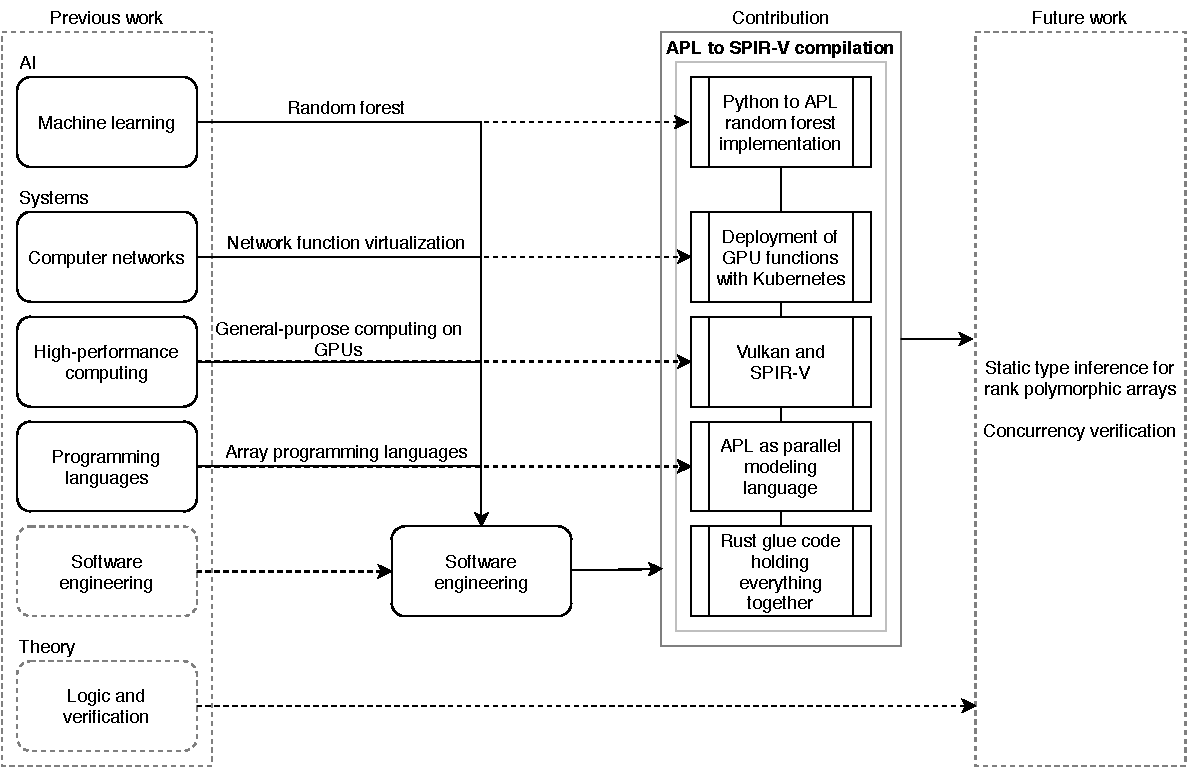
\includegraphics[width=\columnwidth]{./assets/overview.pdf}
  \caption{High-level overview of the research done in this study, and how they relate to previous work}
  \source{\cite{gpupoly}}
  \label{fig:ov}
\end{figure}

The background of this work is convoluted because it combines various aspects of otherwise loose research areas. In hopes to simplify this chapter, a diagram from our previous work Fig. \ref{fig:ov} is presented. In this current work, everything else in the figure beside the logic and verification part is background. So, the background is relevant to understand the \emph{motivation} to apply logic and verification. On the other hand, the related work steers what tools from the logic and verification part we decided to use and how. This chapter is presented such that the related work and the background are intertwined in the text. This was done because the amount of things that contribute to our approach is vast, and at times overlapping between each other, yet still not overlapping with everything. As such, handling background and related work in parallel seemed to results in a more coherent text.

As noted, the motivation of this thesis work stems from our previous work done in \cite{gpupoly}. In the study, we created a GPU program bootloader for a machine learning application in \gls{NFV} domain. While the software artifact worked successfully, the SPIR-V language posed an unexpected challenge. This has to do with type systems for array programming languages. In particular, compiling of compute kernels (\gls{GPGPU} programs) require array types (rank and dimension: together called \emph{shape}) to be known after each operation. When writing the previous report, we adhered to this restriction by manually defining the intermediate types. However, manually defining the intermediate types makes the program inflexible because the input shape must be constant. In other words, if, e.g., the input parameter length changed, the program would not run. We concluded that to make the typing dynamic, an algorithm for \emph{static rank polymorphism} should be developed, which does the following:

\begin{enumerate}
    \item Resolve intermediate types
    \item If a type cannot be resolved, then create a subprogram \emph{phase} with only well-typed calls
    \begin{enumerate}
        \item Then, return the results of the \emph{phase} to CPU for marshaling from the GPU
    \end{enumerate}
    \item Go to the first step until the end of the program
\end{enumerate}

But, to understand what is a shape and what is rank polymorphism, one needs first to understand what APL is.

\section{APL}

The language we used in our previous study to model parallelism was APL. APL is often considered the canonical array language. The trademark of the APL strain languages is the abstraction of mathematical operations. Usually, mathematical operations are represented by a single character Unicodes (such as \verb|⍣⍋⍝⌺|), making the language very terse. The reasoning for such an approach stems from the inventor of APL and a Turing Award laureate, Kenneth Iverson, who created APL as a language to teach matrix algebra in the 1960s. Later on, Iverson went to work at IBM, where his notation was turned into a programming language. Yet, APL lives to date: while its notation is widely considered esoteric, its domain-specificity in mathematical operations remains the basis of modern machine learning libraries, such as Python's NumPy. APL also persists as a domain-specific modeling language for parallel programmers. This is because APL repels constructs that diverge from parallel computation principles: array programming's central idea, \emph{rank polymorphism}, relates to avoidance of explicit recursion and if-clauses (i.e., thread divergence), which forces the programmer to write parallel code by default. This coincides with how APL forces us to think from an array-only mindset, coined as "notation as a tool of thought" \cite{iverson2007notation}, which may produce unconventional but highly parallel algorithms for existing problems. Yet, the idea of terse notation and implicit loops producing parallel code certainly was not planned: the first commercial off-the-shelf multi-core systems came to existence almost half a century later after the invention of APL. This coincidence, in part, makes APL an exciting research topic. It is timely as well: the current decade is seeing an increased proliferation of the use of specialized parallel computers, GPUs, to do computation that does not scale on CPUs anymore. Oftentimes, such application relates to machine learning, in which \emph{array programming} is in a central piece.

As noted above, compared to today's programming languages, APL is distinctively different by abstracting away loops. It also disallows any other data structure than an array. The usual ways of constructing a record, or an object, or a struct do not exist. APL is also read like Arabic, from right to left. Next, we demonstrate APL. In the examples, the input is indented, and the output is not. According to a video\footnote{\url{https://www.youtube.com/watch?v=_DTpQ4Kk2wA&t=122s}}, this is to make it easier to distinguish the output source. We follow the same approach in the following demonstrations, as it remains the default output mode of Dyalog APL. First, single-valued numbers are scalars in APL:

\begin{verbatim}
      9
9
\end{verbatim}

A set of scalars is a vector:

\begin{verbatim}
      9 9
┌→──┐
│9 9│
└~──┘
\end{verbatim}

Operands are called \emph{monadic} when a single argument is given. E.g., \verb|⍴| prints us the \emph{shape} of the argument, e.g., the length for a vector:

\begin{verbatim}
      ⍴ 9 9
2
\end{verbatim}

Another example is the \verb|⍳| which gives the integers from $1..N$ where $N$ is the argument:

\begin{verbatim}
      ⍳9
┌→────────────────┐
│1 2 3 4 5 6 7 8 9│
└~────────────────┘
\end{verbatim}

Operands are said to be \emph{dyadic} when two arguments are given. It is worth noting that two is the maximum amount of arguments that can be provided for any operand in APL. An example of a dyadic operation is the addition:

\begin{verbatim}
      1 + 1
2
\end{verbatim}

Operands have varying functionalities depending on the shape of the argument(s). This functionality is similar to operator overloading in more common languages, such as C++. E.g., (scalar $+$ vector) addition adds the scalar to each element of the vector:

\begin{verbatim}
      1 + ⍳9
┌→─────────────────┐
│2 3 4 5 6 7 8 9 10│
└~─────────────────┘
\end{verbatim}

We also see that the computations are chained automatically. It is also worth pointing out that here, an implicit loop was constructed for the programmer. Next, some other examples where operands are chained. E.g., reduce (\verb|+/|) sums all the elements of an array:

\begin{verbatim}
      +/ ⍳9
45
\end{verbatim}

The "inverse" of a reduction is a scan:

\begin{verbatim}
      +\ ⍳9
┌→──────────────────────┐
│1 3 6 10 15 21 28 36 45│
└~──────────────────────┘
\end{verbatim}

Yet, APL's power, \emph{rank polymorphism}, starts to become more apparent only at higher ranks, such as that of a matrix:

\begin{verbatim}
      3 3 ⍴ ⍳ 9
┌→────┐
↓1 2 3│
│4 5 6│
│7 8 9│
└~────┘
\end{verbatim}

Here, we can see that the functionality of the \verb|⍴| changed when it has arguments on its left and right-hand side. This dyadic form defines that we want to create a 3x3 matrix from the values we get from \verb|⍳ 9|. Next, we can see that the addition operation still works:

\begin{verbatim}
      1 + 3 3 ⍴ ⍳ 9
┌→─────┐
↓2 3  4│
│5 6  7│
│8 9 10│
└~─────┘
\end{verbatim}

And surely enough, so does the scan, which works row-wise to preserve the functional equivalence of the lower rank operand:

\begin{verbatim}
      +\ 1 + 3 3 ⍴ ⍳ 9
┌→──────┐
↓2  5  9│
│5 11 18│
│8 17 27│
└~──────┘
\end{verbatim}

This is rank polymorphism in action: the same program works across different input classes. When thinking about parallelism, this is what makes APL exciting: the input size and rank can change, yet the program does the same operation without any changes. This is significant with parallelism because it allows us to take one big task, e.g., our 3x3 matrix, and \emph{automatically} divide it to, e.g., three smaller tasks, and still run the same program on each core. This way, we get \emph{task decomposition for free}.

\section{Type Systems for Parallelism}

Considering related work, type systems for parallelism could be considered to be closely related with the concept of \emph{shapely types} \cite{jay1994shapely, shkaravska2007polynomial}. Traits of the concept have been recently captured in works related to APL. In \cite{hsu2019phd} a GPU code generating compiler is integrated with the proprietary Dyalog APL implementation. The implementation makes use of the parallel OpenCL backend. In \cite{Henriksen:2016:AGT:2975991.2975997} a subset of APL is typed and compiled into a language called Futhark, which runs on parallel hardware like GPUs via OpenCL, CUDA, and Vulkan backends.

\emph{Static} rank polymorphism can be considered an approach to capture the notion of shapely types. Recently, the subject has been studied in Northeastern University \cite{slepak2014array, slepak2019semantics, shivers2019introduction}, University of Oxford \cite{gibbons2017aplicative}, and University of Copenhagen \cite{henriksen:phdthesis}. These approaches involve dependent types: at Northeastern, they have their language called Remora, at Copenhagen sized-types (a fragment of dependent types) are utilized on their language Futhark, and at Oxford, dependent Haskell was used. Recent industry work can be found from Google as Dex \cite{paszke2021getting}, which proliferates typed indices.

Regarding this work, it quickly became evident that the rational decision to capture static rank polymorphism should follow the general direction pioneered by the related work. As such, we settled with dependent types. And rather conveniently for us, almost as if by plan, the continuation institution after the previous thesis work became the University of St Andrews. This coincides with the place where the dependently typed language \emph{Idris} is developed. As such, it was both logical and convenient to choose Idris as the language for this thesis work. Further, Idris bears some novelty to the previous works: Idris can also be used as a theorem prover like Agda and Coq. This allows theorem prover capabilities to be used, well, to prove properties such as \emph{completeness} and \emph{soundness} pragmatically, i.e., without us coming up with the type system on our own.

\subsection{GPUs as Parallel Processors}

GPUs are arguably the most ubiquitous special-purpose parallel processors. Historically, GPUs have been used to only display pixels on a screen. Since the framebuffer of an operating system is a pixel matrix, the GPU became a specialized yet common hardware piece in modern computers that deals with matrix data. Throughout the years, several abstractions to display 3D content on the screen have appeared in the form of graphics \glspl{API}. These APIs deal with the problem \emph{how} to run a \emph{kernel} (a GPU program) on the device. Recently, these APIs started to have interfaces that allow the GPU to be used for general computation. So, instead of doing computation on the CPU, the CPU can send the data to the GPU, which does the work for the CPU without producing graphics as a side-effect. This method is called \gls{GPGPU} and is a common scaling approach for large datasets often met in applications of machine learning. It could be considered that GPGPU did not see much proliferation until the 2010s and possibly even the latter half of it -- only then did consumer-grade graphics cards start to have meaningful machine learning training throughput, and languages like Nvidia CUDA to support applicable results started to appear. In general, the GPGPU language space is still rather nascent.


\begin{figure}
  \centering
  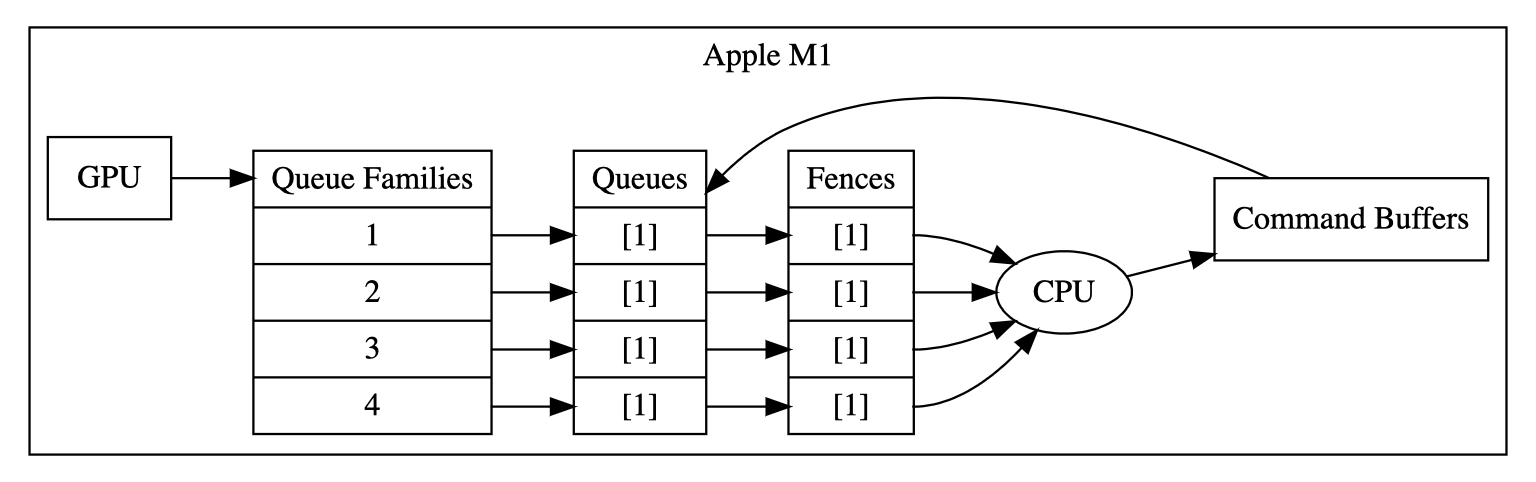
\includegraphics[scale=0.25]{./assets/m1.png}
  \caption{Simplified representation of the Apple M1 system-on-chip device. Important features: GPU and CPU share the same processor. There are four queue families which only have a single queue each. This design allows low latency but has relatively low throughput: the queue count can bottleneck the device if many command buffers are submitted in parallel. The die size of system-on-chips is also smaller, making it physically hard to compete with throughput with discrete graphics cards.}
  \label{fig:m1}
\end{figure}

\begin{figure}
  \centering
  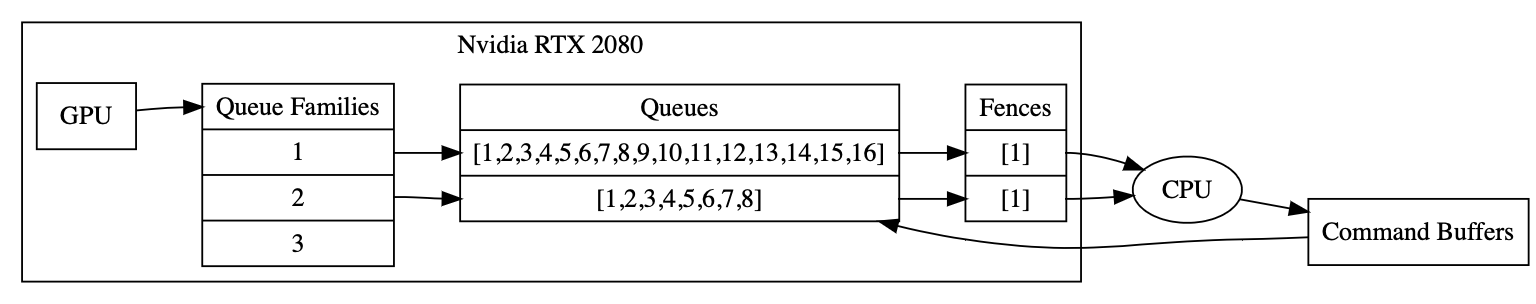
\includegraphics[scale=0.25]{./assets/rtx.png}
  \caption{Simplified representation of the Nvidia RTX 2080 discrete GPU. Important features: GPU and CPU are different processors, so communication between the two happens via the relatively slow PCIe lane. There are two compute-capable queue families which have several queues each. This design has high latency but high throughput: much work can be queued in parallel if the CPU has the cores to do it, but the PCIe lane can be a limit for large datasets. But, when the kernel does get started, the device outperforms commercial off-the-shelf GPU system-on-chips in performance.}
  \label{fig:rtx}
\end{figure}

GPGPUs bring scaling to array processing by the optimized physical structure of the processor. The general idea is to prefer more cores over smart registers and branch predictors. GPUs also have wider SIMD lanes than CPUs, which means the processing of uniformly structured data such as vectors is more efficient. Some other performance-enhancing particularities include memory hierarchy exposure, in which the programmer must select the scope of memory allocations, e.g., whether memory is visible to a single core, cores in its adjacency, or all of the cores. An example kernel, as seen in Fig. \ref{fig:kernel} shows how kernels are usually dynamically typed. When these kernels get translated into \gls{IR} such as SPIR-V, the type is usually converted into a lax format, as seen on line 42 of Fig. \ref{fig:addition}. To elaborate, instead of passing static sizes of the inputs into the kernel as arguments, the size information is simply left out. Leaving out the shape information simplifies programming and pipelines but also results in various complications. The first one is the introduction of \emph{correctness} issues: any computation which is dynamic in size cannot be checked for shape errors. For example, it could be possible to pass in vectors of different sizes, which would lead to undefined behavior. Another challenge is \emph{performance}: the memory type that holds the array must be uniformly shared. In more familiar terms, this means that untyped variables must have global visibility. Further, should untyped array operations be chained together, the resulting challenge is that the memory size is unknown during runtime. Because GPUs cannot dynamically allocate memory during runtime, the shape of the array cannot change. This can be limiting to computation but also result in various marshaling overheads as the data may need to be introspected to remove blank data.

Performance factors also come into play via various physical properties of the GPUs. Having shape analysis would help to use the various design to full efficiency. On Fig. \ref{fig:m1} and Fig. \ref{fig:rtx} we demonstrate the work submission pipeline of two different kind of GPUs. Here, the major difference is the queue size and the available queue families for computation. When command buffers (parameters) for kernels are submitted to a GPU, a destination queue must be chosen. An optimal algorithm resulting in most \emph{parallelism} would utilize as many queue families as possible by splitting the work in a balanced manner. However, to balance any task into multiple pieces, we must be able to reason about the data structure being distributed. Without a static type system aiding in automated decisions, the distribution is left as the responsibility of the programmer. This leaves the programmer with much unnecessary complexity: the programmer must decide not only \emph{what} to compute and \emph{what} functions to use, but also \emph{how} the functions are communicated to the hardware. This amount of decision granularity would only make sense assuming that the programmer knows how the hardware works, but which is seldom the case nor the point. This is especially true in machine learning, where it is commonplace for algorithm developers to be mathematicians and physicists instead of compiler developers or electrical engineers.

Yet, even without complete shape inference, the industry which utilizes GPUs for computing has found its way. Considering related work, an example of this is in Python libraries, which often handle array data on GPUs. A review article \cite{raschka2020machine} provides historical context: Theano (\cite{bergstra2010theano}, 2010) was a compiler (superseded effectively by TensorFlow) for mathematical expressions in Python. It combined the convenience of an array programming syntax with the speed of GPUs. The language was statically typed\footnote{Catching mismatches in the data's numerical format on Python level, but not shape.} and functional. Theano represented computations as a static computation graph. The graph was compiled and optimized before it could be executed. The compilation could take from multiple seconds to several minutes \cite{raschka2020machine}. TensorFlow (\cite{abadi2016tensorflow}, 2016) improved compilation speed over Theano. Per typing, TensorFlow has no restrictions about the definition of the shape of a tensor. As such, TensorFlow allows the following shape cases:

\begin{enumerate}
    \item rank and dimension are known
    \item rank is known, and \emph{some} component of the dimension is not
    \item rank is known, and \emph{any} component of the dimension is not
    \item rank and dimension are unknown
\end{enumerate}

As we remarked earlier, knowing the shape aids in balanced distribution across a single GPU. But, the same information applies to \emph{which} GPU to use (supposing a single computer has many), and even which of the networked \emph{node} to use. In the Python world, this correspondence has been partially realized. Systems such as Dask sidestep static typing by representing computing, again, as computation graphs to represent the dependencies between tasks. Similar to TensorFlow, the return types might not always be known before the graph is executed. For this reason, the \emph{scheduling} is done dynamically. This implies that the distribution is not necessarily optimal. TensorFlow \emph{compilers} take a slightly different approach: XLA requires the shape to be static. This corresponds with the limitations we remarked about untyped arrays earlier in this section. And similarly, as a result, optimizing compilers like XLA can only be applied to a subset of TensorFlow programs.

\section{Dependent Types}

% theoretical basis (how we got here), current implementations (maybe a table for comparisons, e.g., dependent Haskell, Idris, Granule), difference to widestream languages

% gödel system t

We hope that we have now made a convincing case why static shape analysis is useful. As a checkpoint of this long Chapter, we could now summarize what we have learned so far:

\begin{itemize}
  \item array processing is common nowadays in applications of machine learning
  \item array processing is in increasing amounts offloaded from CPUs to GPUs
  \item the canonical array programming language is APL, which exhibits \emph{rank polymorphism}
  \item \emph{static rank polymorphism} could be useful for balanced work distribution across a single GPU, and possibly across a single node, and a network of nodes
  \item related work has approached static rank polymorphism with \emph{dependent types}
  \item the theoretical basis for static rank polymorphism could be summarized to be about \emph{shapely types}
\end{itemize}

Next, we continue with a section about dependent types and Idris. As a reminder, we chose to use Idris in this work as the language to capture static rank polymorphism.

\subsection{Idris}

Idris is a general-purpose programming language that focuses on dependent types as its main distinctive feature. The main influence of Idris is Haskell. In fact, the Idris paper \cite{brady2013idris} explicitly mentions the motivation of the language to be: \say{What if Haskell had full dependent types?}. According to the paper, full dependent types mean no restriction on which values may appear in types. The Idris 2 paper \cite{brady2021idris} elaborates on this further by stating that precise types may describe assumptions about and relationships between inputs and outputs. This is said to be valuable for \say{reasoning about functional properties, such as correctness of algorithms on collections, termination of parsing, and scope safety of programs.} Of these features, the primary benefits of using Idris in this work remain correctness and termination properties. These are essential aspects when modeling programming languages, as the properties allow us to verify that we covered the cases and only the cases we wanted.

As of the time of writing this thesis in 2021, there exist two versions of Idris: Idris \cite{brady2013idris} and Idris 2 \cite{brady2021idris}. While Idris 2 improves on Idris 1 by introducing linearity of variables, this property remains uninteresting for us given the scope of the thesis work. Therefore, for this and stability reasons, we use Idris 1 in this work. Yet, we stipulate on Chapter \ref{ch:discussion} how quantified linearity may help in theorem proving the correctness of various parallel computing schemes, which this work tangents in a subtle manner but mainly leaves as future work.

Throughout the making of this thesis, the book on Idris \cite{brady2017type} was used as supplementary material. However, much of the book, and the online resources available in general, seem to have a different focus than the work in this thesis. In particular, we use Idris mainly to describe precise types and parametric polymorphism of such types. Further, we are interested in restricting inputs with dependent types. Partly, we do this by requiring implicit runtime proofs. This means most of the features we use revolve around the \verb|Data| definitions than functions or interface definitions. Unfortunately, this information was somewhat scarce online, so much time was spent on figuring out what approach works and what does not.

Nevertheless, next, we demonstrate what we exactly hope to achieve with strong typing. To reiterate, the primary motivation stems from restrictions in GPU computation environments, where the non-existence of shared stack memory and inability to allocate memory at runtime create needs for strong typing. In other words, for a generic compiler, the compiler would need to infer the intermediate types after each operation step until program termination. Considering related work, this problem touches on so-called static memory management, which has been an issue in recent programming language research (e.g., \cite{proust2017asap}).

To start the demonstration in the context of APL, consider vector reduction: it takes an input vector, and sums the values into a single value:

\begin{verbatim}
        +/ 1 2 3 4
\end{verbatim}

This will output 10. For matrices, the reduction is made x-wise and the resulting is raveled:

\begin{verbatim}
        mat
1 2 3
4 5 6
7 8 9

        +/ mat
6 15 24
\end{verbatim}

\begin{figure}
    \begin{lstlisting}
    OpDecorate %vector_data ArrayStride 4
    OpMemberDecorate %vector_struct 0 Offset 0
    OpDecorate %vector_struct Block
    OpDecorate %vector DescriptorSet 0
    OpDecorate %vector Binding 1

    %int = OpTypeInt 32 0
    %float = OpTypeFloat 32
    %uint_4 = OpConstant %int 4
    %vector_data = OpTypeArray %float %uint_4
    %vector_struct = OpTypeStruct %vector_data
    %vector_struct_ptr = OpTypePointer StorageBuffer %vector_struct
    %vector = OpVariable %vector_struct_ptr StorageBuffer
    \end{lstlisting}
    \caption{Typed array in SPIR-V}
    \label{fig:typedspirv}
\end{figure}

Here, the first block shows an example matrix called mat. The second block reduces the matrix into a vector. In mainstream languages, the reduce operation would be typed, e.g., \verb|vector -> scalar| for the vector case, and \verb|matrix -> vector| for the matrix case. However, in the SPIR-V language we target, the language requires that the output variable has exact length declared. So, in SPIR-V the type information has to carry the size, i.e., \verb|matrix[3,3] -> vector[3]|. This requirement can be seen from the SPIR-V instructions that relate to defining a vector variable on Fig. \ref{fig:typedspirv}. Verbosity aside, the main point is on line 10, on which we see the \verb|OpTypeArray| parameters. In specific, the \verb|%uint_4| references a constant integer. This corresponds to the specification\footnote{ \url{https://www.khronos.org/registry/spir-v/specs/1.0/SPIRV.html#OpTypeArray}}: \say{Length is the number of elements in the array. It must be at least 1. Length must come from a constant instruction of an integer-type scalar whose value is at least 1.}

Thus, the challenge this thesis work proposes is about typing the length of the array. Further, the problem is not merely about resolving the type initially but on all instructions between the initial and final states. In other words, the type is polymorphic during the execution. In APL, the polymorphism is always well-defined. I.e., the thing that matters for a vector is its length. For a matrix, the dimensions (rows, stride) are significant. However, we can model all the ranks as a single data structure, which we call Shape. This is also nice for generalization reasons. We present our definition of Shape in Fig. \ref{fig:shape}.

\begin{figure}
\begin{lstlisting}[language=Haskell]
    mkRank : (len: Nat) -> (stride: Nat) -> Fin 3
    mkRank len s = case len > s of
      True => the (Fin 3) 2
      False => if (len > 1) then the (Fin 3) 1 else the (Fin 3) 0

    data Dim: (rows, stride, len: Nat) -> Type where
      MkDim: (rows, stride: Nat)
        -> {auto NZs : So (stride > 0)}
        -> {auto NZs : So (rows > 0)}
        -> Dim rows stride (rows * stride)

    data Shape: (rank: Fin 3) -> Dim rows stride len -> Type where
      SomeScalar:
        Shape
          (mkRank 1 1)
          (MkDim 1 1)
      SomeVect:
        (stride: Nat)
        -> {auto NZs : So (stride > 0)}
        -> Shape
            (mkRank stride stride)
            (MkDim 1 stride)
      SomeMat:
        (rows, stride: Nat)
        -> {auto NZs : So (stride > 0)}
        -> {auto NZs : So (rows > 0)}
        -> Shape
            (mkRank (rows * stride) stride)
            (MkDim rows stride)
\end{lstlisting}
\caption{Our polymorphic shape type}
\label{fig:shape}
\end{figure}

On line 12, we have the \verb|Shape| type. The type signature is read as follows: the first argument to \verb|Shape| is called rank, which is of type \verb|Fin 3|. \verb|Fin 3| corresponds to the set of natural numbers that are strictly less than 3. Next, the second parameter must be of type \verb|Dim|. The \verb|Dim| type in itself requires three parameters: rows, stride, and len. From line 6, we can see that these variables are natural numbers \verb|Nat|. On lines 8 and 9, we can also see that the sole constructor of the \verb|Dim| data structure, called \verb|MkDim|, requires implicit runtime proof that stride and rows are greater than 0. If and only if \verb|MkDim| allows so, can a \verb|Dim| be created and.

We have now covered the first line of the \verb|Shape| definition. The next lines of our interest are 13, 17, and 23. On these lines, the constructors for scalars, vectors, and matrices are defined (called \verb|SomeScalar|, \verb|SomeVect|, \verb|SomeMat| respectively. This stresses the previous notion that we do not care about \emph{what} values these corresponds to, just the shape). The most important part is noticing that we are now effectively considering all data formats to be matrices. E.g., on lines 14-16, we can see that scalars are, in fact, just matrices under special conditions. To differentiate these special conditions, the \verb|mkRank| function on lines 1-4 is used. This function declares a rank (of type \verb|Fin 3|) for each \verb|Shape|. The declaration is a bit hard to read, but in effect, the scalars are defined as matrices with a length of 1. Vectors are defined as matrices that have equal length and stride. This implies that matrices are arrays with more than a single value and must have at least two rows (implied by the stride being less than the length of the array).

In effect, by having the \verb|Shape| be the singular data structure to represent all plausible ranks of our APL fragment, our type system only ever needs to pattern match a single data structure. This simplifies the code a lot and solidifies the notion that rank polymorphism is about the shape (rank and the dimensions) of the array, not the values\footnote{Though, no rule without exceptions. An exception of this is filter operation.}.

\subsection{Idris compared to Go}

But why Idris? Cannot the \verb|Shape| be represented in some other language? To entertain this thought, consider a recent programming language with an elementary type system, such as Go. In Go, we can model the same Shape type as mentioned previously with roughly as such:

\begin{lstlisting}[language=Go]
    type Rank int

    const (
        Scalar Rank = iota // Scalar = 0
        Vector             // Vector = 1
        Matrix             // Matrix = 2
    )

    type Shape struct {
        rank Rank
        rows, stride, len uint
    }
\end{lstlisting}

While equivalent on the type level, the challenge becomes with pattern matching the Shape against allowed instructions. For example, a vector reduction in Idris can be modelled as so:

\begin{verbatim}
Reduce : Shape q (MkDim (S r) (S n)) -> Phase
Reduce {q=FZ} o = MkPhase Slash o (mkPar 0 0)
Reduce {q=FS(FZ)} {n} o = MkPhase Slash SomeScalar (mkPar (S n) 0)
Reduce {q=FS(FS(FZ))} {r} {n} o = MkPhase Slash (SomeVect (S n)) (mkPar ((S n)*(S r)) 0)
\end{verbatim}

This is our complete definition which we cover in more detail in the next Chapter, but here, what is needed to understand is that the first line defines the function type signature. The next three lines define "versions" of the function, which corresponds to certain ranks. For example, the line with \verb|{q=FZ}| means that if the rank is 0, then the definition on that line should be used. The next line only applies to vectors and the last one for matrices. Consider the last line. We can see a part that tells \verb|(SomeVect (S n)|. This means, in effect, that a \verb|Reduce| operation for rank two shapes (matrices) modifies the shape by making it some vector of length n. The \verb|(S n)| part checks that the operation can only be done for vectors longer than 0 elements. With Go, we can do this roughly as so:

\begin{lstlisting}[language=Go]
    func (s Shape) Reduce() (Error, Phase) {
      var p Phase = {
        Slash,
        (Reduce s),
        (mkPar s)
      }
      var err Error
      switch s.rank {
        case 0, 1:
          err = errors.New("shape mismatch")
        case 2:
          err = nil
      }
      return err, p
    }
\end{lstlisting}

There is no strict restriction on applying the function against a particular ranked Shape in Go's case. The difference with Idris could be considered categorial: in Go's case, the function exists in the universe of Shape of all sizes, whereas with Idris, a different function exists in the universe \emph{depending} on the rank of the Shape. Thus, while the functional equivalence of the approaches is the same, with Idris, the application is slightly more refined.

\subsection{Idris compared to Rust}

Putting Go aside, other recent languages like Rust provide some features that land somewhere between Go and Idris. In general, Rust can be considered a novel systems programming language with affine types. It promises to overcome the tradeoff between high-level safety guarantees and low-level control over resource management \cite{jung2017rustbelt}. Pure Rust programs are guaranteed to be free of memory errors (dangling pointers, double frees) and data races, without the need of a garbage collector \cite{matsakis2014rust, wang2018krust}. This can be achieved by Rust's affine type system, which implements ownership, moves, and borrows. The unique owner of an object can hand ownership off to a new owner, but the owner may also hand off borrowed references to (or into) the object. These so-called borrows obey lexical scope, ensuring that when the original reference goes out of scope, there will not be any outstanding borrowed references to the object ("dangling pointers"). This implies that when the owner goes out of scope or is deallocated, the referenced object can be deallocated at the same time \cite{matsakis2014rust}. The compiler does this work, and unless the checks pass, the program will not compile.

Rust is an exciting language to model APL, but Rust includes an unsafe block keyword. In Rust, unsafe operations are encapsulated inside specific blocks, which tell the compiler that the programmer is explicitly \emph{circumventing the compiler and the type system}, making the compilation forcibly pass. So, the problem here is that while Rust employs a robust ownership-based type system, it is actually an extension on libraries that internally use unsafe features \cite{jung2017rustbelt}. And with further research, we find that the "no unsafe" macro does not propagate through dependencies, effectively nulling the macro's usefulness in our use case. Thus, we could say that because Rust's type soundness has not been formally proven, there is a good reason to question whether the security properties hold. At least according to one report \cite{matsakis2014rust}, they do not.

However, we could entertain the thought of putting the soundness argument aside and instead focus on the type system expressivity. While Rusts' type system novelty lies in affine types, it has recently gained features towards dependent types, starting from a feature called constant generic types\footnote{\url{https://blog.rust-lang.org/2021/02/26/const-generics-mvp-beta.html}}, which could be considered quasi-dependent types. This is interesting, as some non-academic related work has also appeared between our previous work and this current thesis: a Stockholm-based game company released a project called RustGPU\footnote{\url{https://github.com/EmbarkStudios/rust-gpu}} which implements a SPIR-V fragment in Rust. This way, a programmer can write Rust code and generate SPIR-V code from it. Furthermore, the project leverages the multiple compiler passes of Rust (called MIR\footnote{\url{https://blog.rust-lang.org/2016/04/19/MIR.html}}) to integrate the translation process into the language. As such, this is of significant interest to our effort, as the project would allow us to partially answer to our research objectives using an existing \emph{imperative} language. This is a stark difference to the other related work, which approaches SIMD programming with a functional approach.

To demonstrate constant generic types, we show constant values to be defined for static types. E.g., we can create a type wrapping a pair of arrays of the same size:

\begin{verbatim}
    struct ArrayPair<T, const N: usize> {
        left: [T; N],
        right: [T; N],
    }

    impl<T: Debug, const N: usize> Debug for ArrayPair<T, N> {
        // ...
    }
\end{verbatim}

Similarly, and more interesting to our use-case, type level morphology where the length of the vector is reduced by one element can be described as so:

\begin{verbatim}
    fn split_first<T, const N: usize>(arr: [T; N]) -> (T, [T; N - 1]) {
        // ...
    }

    fn generic_function<const M: usize>(arr: [i32; M]) {
        // ...
        let (head, tail) = split_first(arr);
        // ...
    }
\end{verbatim}

And more importantly, in Rust, should the length of the arr be 0, the compiler will catch this exception and be unwilling to compile the program. The limitation, however, is that this will not prove properties of values that are not constant. Reflecting on our use-case, this would be fine when considering ranks only, but expressing more complicated requirements, such as the implicit runtime proofs, \verb|So (stride > 0)| or static versions of these \verb|Not (stride = 0)| cannot be caught in general (hence the name const generic), unless an example of such natural number value case is provided to Rust, e.g., in the form of a unit test. In Idris, if we do such a requirement for some data type, any function that uses the data type must prove that the argument satisfies this property. E.g., consider:

\begin{verbatim}
    data Dim: (rows, stride, len: Nat) -> Type where
      MkDim: (rows, stride: Nat)
        -> {auto NZs : So (stride > 0)}
        -> {auto NZs : So (rows > 0)}
        -> Dim rows stride (rows * stride)
\end{verbatim}

The NZs proofs could then be provided to some function, e.g., with:

\begin{verbatim}
    Reduce : Shape q (MkDim (S r) (S n)) -> Phase
\end{verbatim}

Here, \verb|(S r)| makes it imperative that the \verb|r| (which is of type Nat) is non-zero value because the definition of \verb|S r| corresponds to a successor of some \verb|Nat n|. The smallest natural number being 0, the \verb|S| of 0 is always at least 1, thus the proof is successfully provided.

Implementation wise Idris provides a slight refinement over Rust, allowing us to reason about propositions over variable types, i.e., non-constant values. This way, reflecting this all to SPIR-V, we enable elementary type inference required by the language and type safety at large.

\section*{Summary}

Static interpretation over types' value ranges remains a unique feature of dependently typed languages such as Idris. When it comes to proving software implementations' properties, Idris can express more strict requirements than general programming languages. We compared Idris to Go and Rust, which has varying levels of type-level expressivity. While some of the functionality we aim for is possible to be programmed at both Go and Rust, the more strict the requirement, the more fragile these imperative languages become compared to Idris's functional style. Thus, it could be concluded that per our initial objectives, Idris is a fine choice.

\chapter{Modeling APL in Idris}
\label{ch:contribution}

The primary artifact of this thesis work is an Idris program which is used to satisfy the challenges laid out in the MSc project specification. Thus, this Chapter is sectioned as follows: System Overview (§\ref{sc:sys}) gives the general idea of how we can use Idris to extract the information we need. Type Safety (§\ref{sc:type}) elaborates on how Idris can be used to reason about data structures such as the rank polymorphic array. Parallelism Modeling (§\ref{section:parmodeling}) section deals with a possible approach to abstractively define parallelism to be used for scheduling schemes for GPUs.

In this study, we define static APL as shape analyzed APL. The array shape information (row count, stride, length) is interpreted separately and ahead of the actual data computation. This way, a programmer could know beforehand when some APL program will run into an error instead of waiting for the program to crash eventually. While interpreted non-static APL has been the standard for much of the complete existence of the language, the previous Chapter mentioned how dependent types are gaining interest as an approach to capture rank polymorphism statically.

Idris is dependently typed language, which includes a termination checker. Thus it can be used as a proof assistant. We showcase in this Chapter how static rank polymorphism can be modeled with Idris' capabilities. We only model the shape morphology, not the data effects of APL operands.

\section{System Overview}
\label{sc:sys}

As we are modeling APL, it affects the way we architecture the Idris code significantly. In specific, APL is a language with quirky limitations: each function is either a \emph{monadic} or \emph{dyadic}. Monadic means the function takes only a single argument, whereas dyadic functions take two. Arguments are always polymorphic arrays. Polymorphism means a transformation of one set into another that preserves in the second set the relations between elements of the first. In the context of APL and arrays, each rank of an array can become a rank of some other dimension. The ranks which this work defines correspond to those available in the classical APL form of the 1960s, which means support for scalars (rank 0), vectors (rank 1), and matrices (rank 2).

\subsection{The Type System}

Introducing a type system for APL might be confused or associated with introducing explicit types to APL\footnote{In particular: \emph{Does APL Need a Type System? by Aaron W Hsu at \#FnConf18} - \url{https://www.youtube.com/watch?v=z8MVKianh54}}. But, this is not our objective. Instead, the idea is to retain APL as APL and introduce a separate type-checker procedure which infers the possibility of type errors \emph{implicitly}. This is mainly possible because APL is predictable, with its limitation of 1 or 2 arguments and linear execution direction. However, because a single APL program might work on any ranked array, it is also possible that some programs require the inputs to be of specific parameters. In these cases, whether the program is safe to run or not will only be known when the parameters are known. So, the type-checker will accept a program if it may work for at least \emph{some} rank, but whether it works for a particular input is always dependent on the type-checker to be re-run in respect of those parameters. E.g., \verb|{0 1 = ⍵}| is an APL program that only works on shapes that are rank one and of length 2. Meanwhile, programs such as \verb|{1 = ⍵}| apply to any rank\footnote{While not further studied in this work, it would be interesting to research the category of APL programs that do not have constant array expression in them but are still limited to a certain rank, and that such limitation can be captured statically independently of parameter evaluation.}. This kind of type of system aid could be engaging in an \glspl{IDE}: if the applicable ranks could be shown for a piece of APL program, would the programmer instead make a generic program more strict, or a strict program more generic?

As another example, suppose we have the program \verb|{1 + ⍵}|. To check for its type-safety, we run an intermediate parser and interpreter, which translates this to our Idris version: \verb|Sum (SomeScalar) (_input?)|. Once the argument is given, then the input part is filled, and the Idris code is run. If the result is an error, we do not attempt at the actual execution, but otherwise, the program is run on the GPU using the program bootloader we made earlier in \cite{gpupoly}. While we did not provide the parser and interpreter part in this study, we note it is possible to re-use related work with minor modifications, such as ivy\footnote{\url{https://github.com/robpike/ivy}}. As such, the type system is transparently added atop APL. Programs with type errors can be caught even though no additional typing is added into the APL source code. This could be interesting for educational purposes as well, as noted later in §\ref{sc:dependentapl}.

\subsection{Polymorphism}
\label{section:polymorphism}

It could be said that most people familiarize polymorphism with object orientated programming. Here, subclasses can define their functionality while still preserving the functionality of the parent class. Yet, the same kind of polymorphism can also be captured in functional programming languages with dependent types, such as Idris. Specifically, in Idris, we can restrict the applicable set of functions of an arbitrary datatype $T$:s instances $t$ by $t$'s value. For example, and in specific with ranks, let $T$ be a datatype which first and the only parameter is the finite field of natural number 3. Now, of $T$ we can create an instance with \verb|t = T (FS (FZ))|, i.e., here $t$ gets a value of 1. Next, we can define functions which are \emph{dependently typed} to require the first parameter to be $T$ with a \emph{value} of 1. E.g., suppose such function is named $f$. Now, the accepted parameters of $f$ are restricted to only such instances with the value of 1. As such, $f$ applies to the recently created variable $t$, as $t$'s first and only constructor's value is 1. Would we now redefine $t$'s value to match 0, i.e., \verb|t = T FZ| , $t$ would not no longer be in the universe of function $f$, and as such, attempt to apply $f$ on $t$ would result in a type-error. In code:

\begin{lstlisting}[language=Haskell]
    data T: Fin 3 -> Type where
      mkT: (ff: Fin 3) -> T ff

    f : T 1 -> Nat
    f t = 1
\end{lstlisting}

Now, \verb|f (mkT 1)| results in \verb|1 : Nat|, but \verb|f (mkT 2)| would produce a type-error. It is worth noting that the rank inference can be made dynamic by generic enough constructor. Suppose the Rank datatype defined in Fig. \ref{fig:shape}, with the relevant part being repeated below:

\begin{lstlisting}[language=Haskell]
    mkRank : (len: Nat) -> (stride: Nat) -> Fin 3
    mkRank len s = case len > s of
      True => the (Fin 3) 2
      False => if (len > 1) then the (Fin 3) 1 else the (Fin 3) 0
\end{lstlisting}

If the function is used on each constructor under Shape, it allows automatic refinement of types into stricter versions. E.g., see:

\begin{itemize}
  \item \verb|SomeMat 1 1|, which returns:
  \begin{itemize}
    \item \verb|Shape FZ (MkDim 1 1)|
  \end{itemize}
  \item \verb|SomeVect 1|, which returns:
  \begin{itemize}
    \item \verb|Shape FZ (MkDim 1 1)|
  \end{itemize}
  \item \verb|SomeScalar|, which returns:
  \begin{itemize}
    \item \verb|Shape FZ (MkDim 1 1)|
  \end{itemize}
\end{itemize}

In other words, even if the constructor for vector or matrix is used, but the input corresponds to a scalar, then the identity of a scalar is returned instead of vector or matrix. The equivalence interface between the type would thus correspond to equivalent rank and dimension.

To recap, we can say that we achieved polymorphism in two ways: one via the more classical object-orientated way where we limit the applicability of some data structure by creating dependently typed methods for it, and the second by generalizing the Shape datatype creation to be applied to each plausible rank, and allow easy propagation for refinements. Now, if we want to create some Shape, we can always be explicit and use the \verb|SomeMat| constructor, or we can be more implicit in the rank and use \verb|SomeVect| for vectors and \verb|SomeScalar| for scalars. Arbitrarily higher dimension arrays could be created by vectorizing the \verb|Dim| datatype. E.g., cuboids (vectors of matrices) would be \verb|Shape 4 Vect 2 Dim row stride len|, and so on. Nested arrays we can posit to be vectors of shapes: 2x3 matrix where the second column is a 3x3 inner matrix would be \verb|Vect 3 Shape r Dim row stride len|, where the values are:

\begin{enumerate}
    \item \verb|Shape 2 Dim 2 1 2|
    \item \verb|Shape 2 Dim 6 3 18|
    \item \verb|Shape 2 Dim 2 1 2|
\end{enumerate}

A cuboid of an inner matrix would become a pretty complicated structure, which makes for an interesting future study in an attempt to capture it all in a single Shape constructor. In the following subsection, we see why the Shape is also essential to be returned by all operations.

\subsection{Shape Applicability}

\begin{figure}
\begin{lstlisting}[language=Haskell]
    data Operation =
      Plus | Minus
      | Slash | Backslash
      | Equal ... and so on

    data Parallelism: Nat -> Nat -> Type where
      mkPar: (x: Nat) -> (y: Nat) -> Parallelism x y

    record Phase where
      constructor MkPhase
      operation : Operation
      shape : Shape rank (MkDim (S rows) (S stride))
      par : Parallelism x y
\end{lstlisting}
\caption{The Phase record allows operation chaining while leaving room for future parallelism modeling.}
\label{fig:record}
\end{figure}

APL operands always return a Shape. Because Shape is polymorphic, APL programs are mutations over a single data structure, $\omega$. The $\omega$ is always the last argument of any APL program, i.e., the innermost variable in the Idris representation. This $\omega$ is carried throughout the program, sometimes interacting with left-side argument $\alpha$, yet still always returning a Shape. In our implementation, we achieved this functionality with records. The Idris code for the record is shown in Fig. \ref{fig:record}. Next, we define functions with the following pattern:

\begin{verbatim}
    f : Shape r (MkDim (S r) (S n)) -> Phase
\end{verbatim}

The Phase return type ensures that we can extract the Shape from the return value. E.g.:

\begin{verbatim}
    shape (Reduce (SomeVect 4))
\end{verbatim}

Which returns the Shape type, as each APL operand should:

\begin{verbatim}
    SomeScalar : Shape FZ (MkDim 1 1)
\end{verbatim}

This allows us to easily chain operations together in Idris:

\begin{verbatim}
    shape (Sum SomeScalar (shape (Reduce (SomeVect 4))))
\end{verbatim}

So, we can chain Shape operations via the Phase record. We query the Shape of the record with the shape keyword, which corresponds to the field name as shown in \ref{fig:record}. If we run this piece of code, a Shape type is returned, as each well-typed APL operand does:

\begin{verbatim}
    SomeScalar : Shape FZ (MkDim 1 1)
\end{verbatim}

In effect, this allows us to construct APL programs of arbitrary length in Idris. We can inspect any intermediate part of the computation to see what the type is. This is what is needed for typing the intermediary values for GPU compute kernels.

\section{Type Safety}
\label{sc:type}

Type safety is a static property. It checks that given some APL program, we can infer that a program would eventually result in a badly typed operation, shape-wise. An example is the Hadamard products: in APL, matrix operations require the terms to have symmetrical dimensions. As current APLs are dynamically typed, some deferred operations on the program flow may cause an exception. With more enormous datasets or more complicated programs, such errors might take time to come up.

As such, complete shape analysis implies strong runtime guarantees. We define \emph{shape analysis} as the ability to carry over a distinct polymorphic shape type and the ability to resolve its definition at each step of the morphology. This analysis is achieved with Idris's dependent type system: each "phase" of the program produces a result type, which is passed to consecutive phases. In our study, phases are abstract models of various APL operands: e.g., a reduce operation has the effect of decreasing the rank of the shape. E.g., a vector is reduced to a scalar and a matrix into a vector. We denote this as abstract, as we are not interested in the values of the data structure but instead focus on the shape, which we model as a flat matrix with stride information.

As already seen before, a reduce operation over a vector has the effect of pruning the vector's length to 1. In code, this can be achieved with the following:

\begin{verbatim}
    shape (Reduce (SomeVect 4))
\end{verbatim}

This will output:

\begin{verbatim}
    SomeScalar : Shape FZ (MkDim 1 1)
\end{verbatim}

The PReduce itself is a phase, defined as so:

\begin{verbatim}
Reduce : Shape q (MkDim (S r) (S n)) -> Phase
Reduce {q=FZ} o = MkPhase Slash o (mkPar 0 0)
Reduce {q=FS(FZ)} {n} o = MkPhase Slash SomeScalar (mkPar (S n) 0)
Reduce {q=FS(FS(FZ))} {r} {n} o = MkPhase Slash (SomeVect (S n)) (mkPar ((S n)*(S r)) 0)
\end{verbatim}

Where MkPhase is a record constructor from Fig. \ref{fig:record}. This allows us to encode parallelism hints to phases while also type checking the APL program in Idris. Consider the APL program, which reduces a vector to a single value and then sums one to it:

\begin{verbatim}
      1 + (+/ 1 2 3 4)
11
\end{verbatim}

In our Idris program, this operation can be encoded with:

\begin{verbatim}
    shape (Sum SomeScalar (shape (Reduce (SomeVect 4))))
\end{verbatim}

This will output:

\begin{verbatim}
    SomeScalar : Shape FZ (MkDim 1 1)
\end{verbatim}

In other words, Idris confirms that the APL operation will return some scalar. Next, let us consider the following APL program:

\begin{verbatim}
      1 2 3 4 + (+/ 3 3 ⍴ ⍳9)
\end{verbatim}

When we try to run the program in Dyalog APL, we get:

\begin{verbatim}
    LENGTH ERROR: Mismatched left and right argument shapes
\end{verbatim}

As we can see, APL will notice this type of error, but under the hood, this is not static analysis. We can see this with a delay function:

\begin{verbatim}
      (1 2 3 4 + (+/ 3 3 ⍴ ⍳9)),⎕DL 10
\end{verbatim}

The added code adds a sleep into the operation. As the delay has no effect on the later program, if static analysis would be employed, then we should immediately see an error. However, what happens is that only after waiting 10 seconds do we see the error re-appear. We can model this in our APL system:

\begin{verbatim}
shape (PSum (SomeVect 4) (shape (PReduceMat (SomeMat 3 3 9))))
\end{verbatim}

\begin{figure}
    \begin{lstlisting}[
        basicstyle=\small, %or \small or \footnotesize etc.
    ]
(input):1:8-54:When checking an application of function Shaped.Sum:
Type mismatch between
    Shape (free_rank (Reduce (SomeMat 3 3)))
          (MkDim (S (free_rows (Reduce (SomeMat 3 3))))
                 (S (free_stride (Reduce (SomeMat 3 3))))) (Type of shape (Reduce (SomeMat 3 3)))
and
    Shape (mkRank 4 4) (MkDim 1 4) (Expected type)

Specifically:
    Type mismatch between
            free_stride (Reduce (SomeMat 3 3))
    and
            3
    \end{lstlisting}
    \caption{An example of a shape error in Idris when trying to sum matrices with mixed dimensions together.}
    \label{fig:shapeerror}
\end{figure}

This will output the error shown in Fig. \ref{fig:shapeerror}. Here, Idris helpfully tells us that a mismatching stride produces the error. In fact, this is the same error as what Dyalog APL is saying. Considering the initial objectives of the research, these features correspond to the capture of runtime errors. The reason this runtime error is captured is explained by symmetric Sum definition:

\begin{verbatim}
    Sum : Shape p (MkDim (S r) (S n)) -> Shape p (MkDim (S r) (S n)) -> Phase
    Sum {r} {n} a o = MkPhase Plus o (mkPar 0 ((S n)*(S r)))
\end{verbatim}

On the first line, we can see that the \verb|MkDim| constructor requires the second argument to be the same. This is identified by the parameter being $n$ in both cases. This signifies to Idris that the value of the type here is supposed to be the same. But, the strides of \verb|(SomeVect 4)| and \verb|(SomeVect 3)| mismatch, so we can capture a shape error.

\section{Parallelism Modeling}
\label{section:parmodeling}

Modeling parallelism on type-level became an evident requirement in the previous thesis work. Further, it was a much more complicated topic than initially thought. In essence, we need knowledge of parallelism in two components: the scheduler and the parallel code. The challenge is that one affects the other: consider a vector with ten values. Suppose you have five cores. Suppose you want to add some scalar, say 1, to each value. You can schedule each of your five cores to own two values, to which each core adds the scalar 1. This works, but we call it the naive method. Next, we demonstrate why:

\begin{enumerate}
    \item Bytecode \emph{vectorization} (i.e., SPIR-V) specific:
    \begin{itemize}
        \item Each GPU core has a SIMD lane which allows certain special operations documented in the SPIR-V specification\footnote{\url{https://www.khronos.org/registry/spir-v/specs/unified1/SPIRV.html#_a_id_group_a_group_and_subgroup_instructions}} to be executed fast. The SIMD lane is a variable across GPU manufacturers, and it \emph{may} be varying between different cores over a single execution. In general, the lower bound for manufacturers is on Intel, which defines the SIMD lane to \emph{usually} have the width of 8 values. The upper bound is usually of AMD's domain, which has SIMD lanes of widths of \emph{usually} 64 values. As such, an optimization rises: one does not need to schedule 5 cores for 10 values if the operation is SIMD-capable. In our example, it is, so we can instead schedule a single core to sum the values using a single call, which likely has lower latency.
        \item A single data value in SPIR-V can be a scalar, vector, or matrix. Vectors and matrices are limited: a vector can have $1..4$ values, and a matrix can have dimensions from $1..4 x 1..4$. This means that a single operation can abstracts SIMD calls over an array of values. What this means is that a single group call on AMD would operate on 64 values which might at most be 4x4 each, making a single opcode effectively operate over $1024$ values at once. However, a decision logic would be needed to figure out when to compose the data into these abstractions, and if so, what lengths to use.
    \end{itemize}
    \item Scheduling (i.e., Vulkan) specific:
    \begin{itemize}
        \item The cores on the GPU, or CPU for that matter, are rarely equal. The GPU is made of various core queue families. A family has different properties and various amounts of queues. For example, an Apple M1 with marketed 8 GPU cores has four queue families, which are all compute capable, but each queue family has only a single queue. As marketing material and what the APIs can parse differentiate, it can easily be the case that even the programmer does not know the hardware's physical properties. On the other hand, Nvidia discrete GPUs tend to have three queue families, of which usually two are compute capable, and a single one is only data-transfer capable. With Nvidia and other discrete GPU manufacturers, the two compute-capable queue families tend to have a varying number of queues in them, usually 16 and 8. The third usually has only one, but this one is a special fast-transfer queue incapable of doing computation. Next, you can submit to multiple queues in parallel, assuming that your CPU has more than a single core. As such, suppose we had 100 values instead of 10. We could assign two cores on two separate queue families to work in parallel. This is beneficial because computation latency is reduced and allows results to be streamed in real-time as they pass a memory fence. This concept, sometimes called async compute, thus effectively allows us to chunk the work into pieces that execute out-of-order and may improve latency.
        \item A single computer might have multiple GPUs with varying queue family capabilities and thread counts. As such, you now need to abstract the above items to consider all GPUs you have.
    \end{itemize}
\end{enumerate}

\begin{figure}
  \centering
  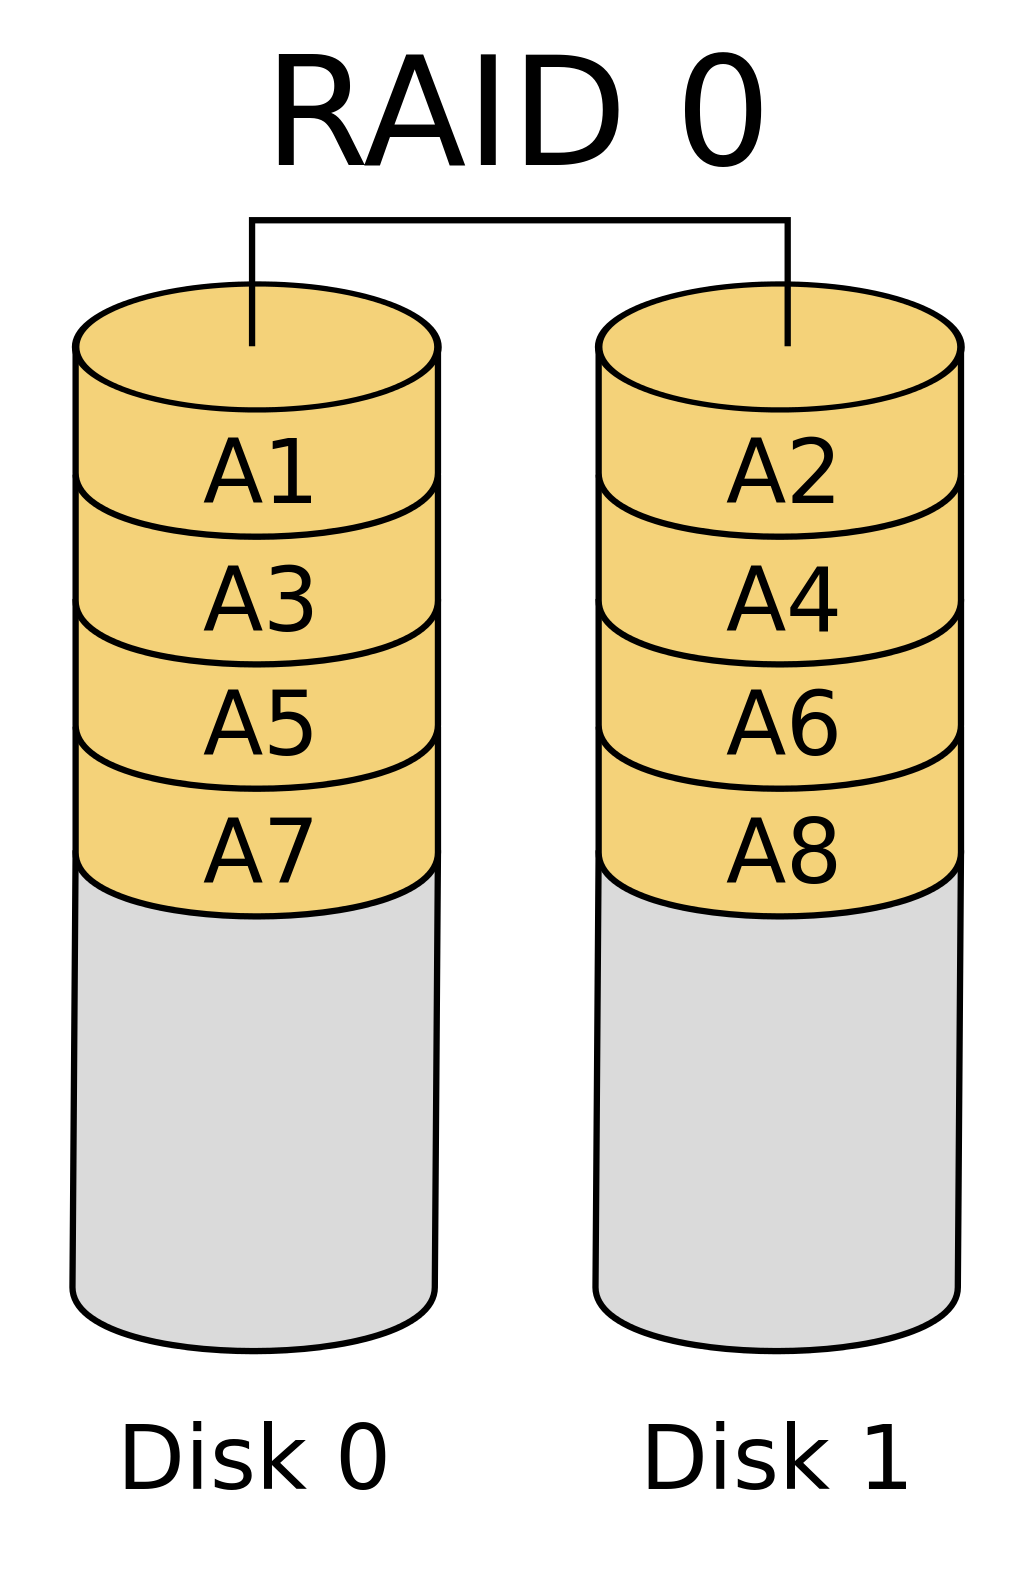
\includegraphics[scale=0.1]{./assets/1024px-RAID_0.svg.png}
  \caption{Diagram of a RAID 0 setup.}
  \source{Colin M.L. Burnett (via Wikipedia)}
  \label{fig:raid0}
\end{figure}

Now, it is worth noting that shape analysis only helps with the scheduling parts. On an abstract level, we can see that the scheduling can be done only with the shape information, whereas the bytecode-specific information is more reliant on data. I.e., the SPIR-V optimizations would also need to know how \emph{some data} is being accessed throughout the lifetime of the program. This is a much harder problem to solve than answering to how \emph{some task} can be spread across many cores. To visualize this difference, we can think about the scheduling work as thinking about RAID layouts. On Fig. \ref{fig:raid0} we can think of what happens with the scheduling of a GPU: because the computation model is SIMD, this implies that the kernels are self-sufficient to do computation. As such, one can distribute the computation over two queue families (captioned as disks on the figure), and the $A\{N\}$ chunks are individual queues. Interestingly, this distribution is very generic because of SIMD: the disks in the figure could represent different GPUs or different computers. More importantly, this captures the principle that \emph{the type system can distribute our computation}. For example, suppose we have a $100x100$ matrix, and we want to sum reduce each row. Suppose we have four queue families with one queue each. To use the queues to our best effort, we can split the $100x100$ into four equal parts. Then, with $25x100$ tasks assigned to each queue, we can further split this work into $25$ commands, which we can submit to the GPU. Once all the work has been submitted, we wait for all the commands to complete. Then, we join the results of each of the \emph{queue family} into a single result. Thus we have our resulting $1x100$ matrix, possibly out-of-order, depending on whether we care about ordering or not. Coincidentally, this shows that we can address the scheduling scheme depending on the task's shape changes and $x,y$ dimensional dependencies. The usefulness of rank polymorphism here is worth noting: we can slice the initial task into smaller subtasks as long as the APL program type-checks. So, even though the programmer created the APL program to work on matrices, most likely, it also works for vectors. If so, i.e., it type-checks, we can automatically subslice the program for asynchronous execution on the scheduler side. If not, we know that there is a data dependence, and we cannot refine the execution further. Though, as it is evident, sometimes we may refine the execution to a single scalar. So, there must be a balancing factor: you do not want to submit too many individual tasks on the CPU side because then the execution will become CPU-bound. On the other hand, if the GPU cannot effectively use its cores (e.g., there will be a high thread-divergence), the job will be GPU-bound. Balancing these factors is a complicated process that we leave as future work. However, some factors that affect this decision procedure are how many queues, and queue families are available, how many memory allocations must be done, and how many CPU cores are needed to submit all the tasks effectively. It is worth noting that there might not be a single correct solution -- some approaches will stress out the computer CPU more than the others, while some might block the GPU entirely from any other tasks. Nevertheless, with APL and a type-system, we can start exploring these strategies, which is progress in itself -- automatic parallelism inferation is no easy task. However, due to the assumptions, we can make about APL, these approaches can be tested.

But what about the bytecode optimization, i.e., vectorization? This comes to the question of the relevance of tracking individual array cell's lifetime. During a literature review, it was found that there exists a form of logic called \emph{dependence logic} which provides models to think about this relation. Per \cite{sep-logic-dependence}: "Dependence logic is an extension of first-order logic which adds to it dependence atoms, that is, expressions of the form $=(x_{1}...x_{n},y)$ which assert that the value of $y$ is functionally dependent on (in other words, determined by) the values of $x_{1}...x_{n}$. These atoms permit the specification of non-linearly ordered dependency patterns between variables". The dependence logic gives us some perspectives on how the data values could be modeled, e.g., team semantics \cite{hodges1997compositional} which posits how some values are dependent on teams of values. This kind of abstract interpretation would give more detail to operations such as vector reduction. Instead of the shape only being modified, we could have a notion which additionally captures the fact that the produced \verb|SomeScalar| is also dependent on the values of the whole vector. This could still be interpreted without overthinking the actual value. However, some proofs could be extracted, e.g., that the \verb|SomeScalar| satisfies the fact that its value is more or equal to any value in the input vector. E.g., we could say in Idris:

\begin{lstlisting}[language=Haskell]
    data Value: Vect n Int -> Int -> Type where
        EQorQT: (vec: Vect n Int) ->
            -> {auto isQT : (count 0 vec) > (len (vec - 1))}
            -> Value (S (max vec))

    reduce : Vect n Int -> Shape [...]
    reduce v = SomeScalar (logicalAND (1 (EQorQT v)))
\end{lstlisting}

So, the point is that on line 7, we do computation on the vector values, but we could always discard the value. This way, we could still check some propositions on the data, and this way carry out proofs during the type-checking of the program. Next, if we would instead carry over the proofs during the program lifecycle, we could catch some redundant execution. Again, whether this has any practical upside would require further studies. However, there could be some exceptional cases in which this could be beneficial for execution: e.g., if two vectors $A$ and $B$ are ordered, and we want to check whether the sum reduction $a$ of $A$ is greater than sum reduction $b$ of $B$, then there would either exists an execution path where $(\square (a>b))$ or vice versa. If these dependence proofs under which these conditions hold could be carried and represented in bytecode, then the execution could pre-emptively stopped. And, it is worth noting that because SIMD computation tends to work in lockstep, i.e., there are separate compute and synchronization steps, then these proofs could be evaluated on the synchronization part and put into practical use.

\begin{figure}
  \centering
  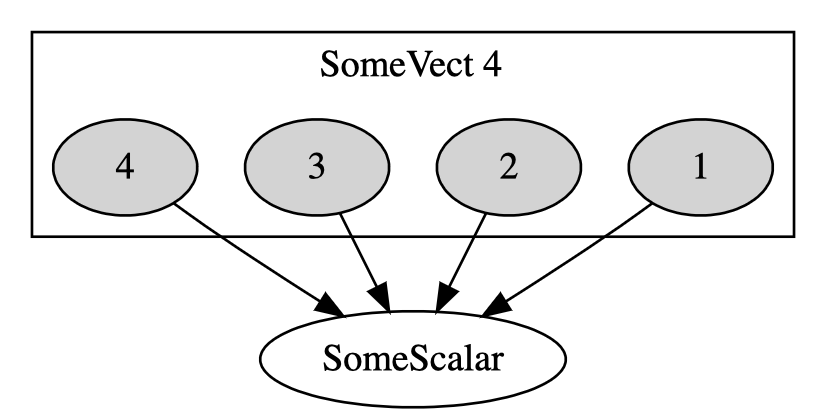
\includegraphics[scale=0.25]{./assets/reduce.png}
  \caption{Visualization of a 4-value vector reduction.}
  \label{fig:reduce}
\end{figure}

\begin{figure}
  \centering
  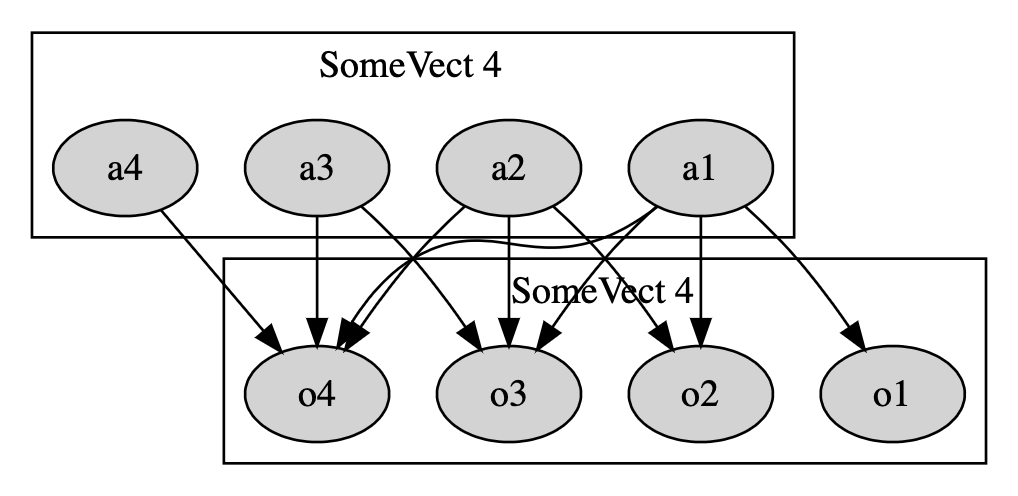
\includegraphics[scale=0.25]{./assets/scan.png}
  \caption{Visualization of a 4-value vector scan.}
  \label{fig:scan1}
\end{figure}

\begin{figure}
  \centering
  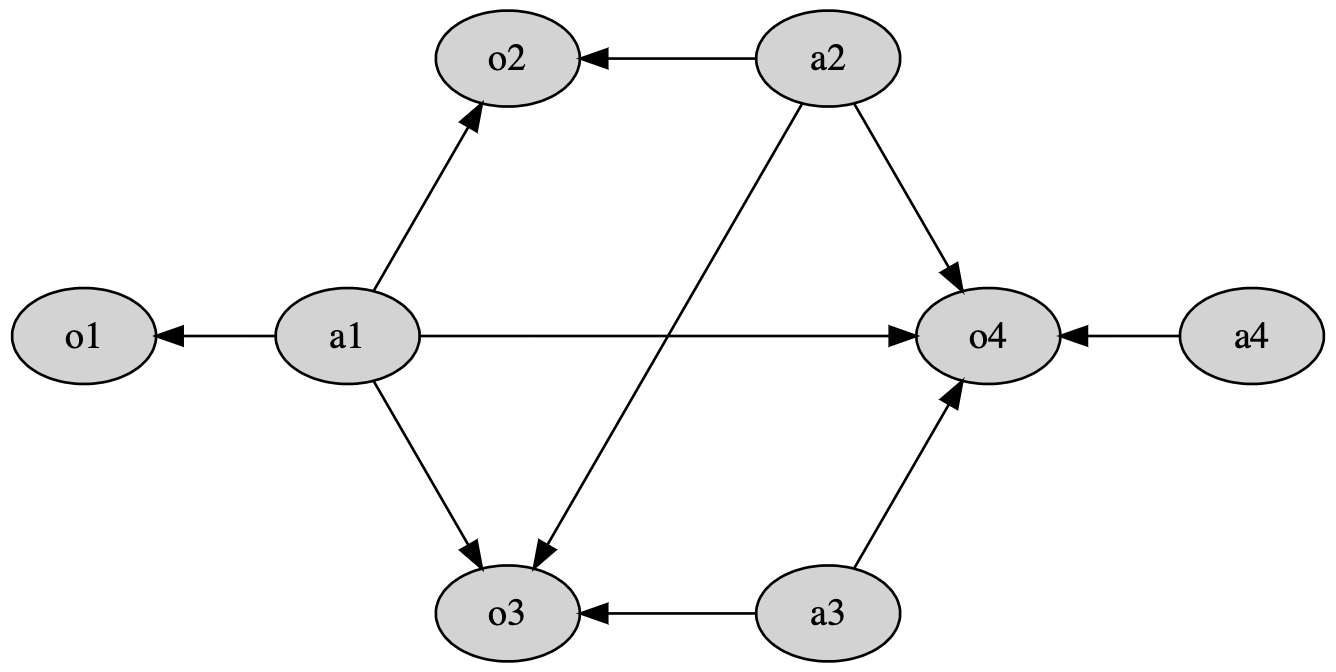
\includegraphics[scale=0.25]{./assets/scan2.png}
  \caption{Alternative visualization of a 4-value vector scan without explicit shape information. $a$ values are starting values, $o$ values are result values.}
  \label{fig:scan2}
\end{figure}

But, effective tracking of single values dependencies might also be a good way to visualize parallelism: implied by the previous example's use of \gls{LTL}, we could model the \verb|Parallelism| part in Idris as automatons. So, instead of saying that we have parallelism in some $x,y$ dimension, we could denote how the values are transformed. This bears extra information over a single integer change: consider the Fig. \ref{fig:reduce}. Here, the model of computation is more precise: it shows that the shape is modified into a scalar by contributing each value independently to the result. Now, consider scan in Fig. \ref{fig:scan1}. This further shows the relation on what values affect what results. The scan figure can also be shown in an alternative format, as seen in Fig. \ref{fig:scan2}, from which we can now more clearly see that which exact values are the bottleneck. Creating this kind of graph model straight from Idris is left for future work because it assumes that the effective scheduling part is solved. It remains unclear whether the branch of dependence logic can affect the parallelism aspects without making too many assumptions.

It is worth noting that this kind of automaton work is similar to the directed graph approaches of our related work in TensorFlow and Dask. However, these systems are limited in expressivity because the types are not known statically. Combining the graph dependence approaches of these works, but now with a static type system, could result in more optimized execution strategies that TensorFlow and Dask cannot do because the languages they target do not have complete shape analysis. Attempting to optimize the graphs with more information could be meaningful for long-running machine learning training. Yet, the effectiveness of such an approach is left for studies of future work, but there does not seem to be a reason why the approach, in general, would not work.

\section*{Summary}

With Idris, we can model the type safety of APL programs by interpreting only the shape changes of a rank polymorphic array. This can be done without introducing any type of semantics to current APL programs. Coincidentally, the shape changes help us in the scheduling of SIMD computations. However, capturing the true potential of SIMD hardware would also require us to reason about the logical dependencies of values, which is left for future work. Yet, it seems that these relations could still be modeled in Idris.

\chapter{Evaluation}
\label{ch:evaluation}

\begin{table*}
\begin{center}
\begin{threeparttable}[b]
\caption{DOER outcomes}
\label{fig:doer}
\begin{tabular}{|p{4cm}|p{2cm}|p{4cm}|p{2cm}|}
\hline
Primary goal
& Primary outcome
& Secondary goal
& Secondary outcome
\\
\hline
Model rank polymorphism: model at least three operations that work on all of the ranks of scalars, vectors, and matrices
& \cmark (§\ref{sc:rankpolym})
& Use Idris to check whether any program created with the implementation is total
& \cmark\tnote{a}
\\
\hline
Catch runtime errors: model at least one APL operand that can cause a runtime error but which can be statically detected
& \cmark (Fig. \ref{fig:shapeerror})
& Use Idris to check whether any program created with the implementation can finally be transformed into a matrix
& \cmark (§\ref{section:polymorphism})
\\
\hline
Termination: ensure termination of functions that operate on the Shape type
& \cmark (§\ref{sc:temination})
& Study how dependent types could model safe parallelism
& \cmark (§\ref{section:parmodeling})
\\
\hline
\end{tabular}
    \begin{tablenotes}
    \item [a] We get no errors when running the source file, despite having \verb|%default total| enabled.
    \end{tablenotes}
    \end{threeparttable}
\end{center}
\end{table*}

A table is provided, Table \ref{fig:doer} in which the primary and secondary objectives are compared to what has been presented so far. Below are sections that further elaborate on the outcomes.

\section{Regarding Termination}
\label{sc:temination}

As noted in the ($^{a}$) footnote of Fig. \ref{fig:doer}, the termination is proven by the use of \verb|%default total| macro in the Idris source files. But, to check that it actually works, we could consider the Reduce function again:

\begin{verbatim}
Reduce : Shape q (MkDim (S r) (S n)) -> Phase
Reduce {q=FZ} o = MkPhase Slash o (mkPar 0 0)
Reduce {q=FS(FZ)} {n} o = MkPhase Slash SomeScalar (mkPar (S n) 0)
Reduce {q=FS(FS(FZ))} {r} {n} o = MkPhase Slash (SomeVect (S n)) (mkPar ((S n)*(S r)) 0)
\end{verbatim}

If we remove the bottom line and re-run the program, we will get an error:

\begin{verbatim}
s2.idr:57:1-54:
   |
57 | Reduce {q=FZ} o = MkPhase Slash o (mkPar 0 0)
   | ~~~~~~~~~~~~~~~~~~~~~~~~~~~~~~~~~~~~~~~~~~~~~~~~~~~~~~
Shaped.Reduce is not total as there are missing cases
\end{verbatim}

As our implementation does not complain about such errors by default, we know that our program is total, thus terminating.

\section{Modeling Rank Polymorphism}
\label{sc:rankpolym}

\begin{figure}
\begin{lstlisting}[language=Haskell]
    -- shape (Reduce (SomeVect 4))
    -- shape (Reduce (SomeMat 3 3))
    -- shape (Sum (SomeVect 4) (shape (Reduce (SomeMat 3 3))))
    -- shape (Sum SomeScalar (shape (Reduce (SomeVect 4))))
    Reduce : Shape q (MkDim (S r) (S n)) -> Phase
    Reduce {q=FZ} o = MkPhase Slash o (mkPar 0 0)
    Reduce {q=FS(FZ)} {n} o = MkPhase Slash SomeScalar (mkPar (S n) 0)
    Reduce {q=FS(FS(FZ))} {r} {n} o = MkPhase Slash (SomeVect (S n)) (mkPar ((S n)*(S r)) 0)

    Scan : Shape p (MkDim (S r) (S n)) -> Phase
    Scan {r} {n} o = MkPhase Backslash o (mkPar ((S n)*(S r)) 0)

    -- shape (Sum SomeScalar SomeScalar)
    -- shape (Sum (SomeVect 4) (SomeVect 4))
    -- shape (Sum (SomeMat 3 3) (SomeMat 3 3))
    Sum : Shape p (MkDim (S r) (S n)) -> Shape p (MkDim (S r) (S n)) -> Phase
    Sum {r} {n} a o = MkPhase Plus o (mkPar 0 ((S n)*(S r)))

    -- shape (NSum SomeScalar (SomeVect 4))
    -- shape (NSum SomeScalar (SomeMat 3 3))
    NSum : Shape 0 (MkDim (S r) (S n)) -> Shape p (MkDim (S j) (S m)) -> Phase
    NSum {j} {m} a o = MkPhase Plus (SomeMat (S j) (S m)) (mkPar 0 ((S j)*(S m)))
\end{lstlisting}
    \caption{Modeled operations: Reduce, Scan, Sum.}
    \label{fig:modeled}
\end{figure}

Considering \ref{fig:modeled}, we can see that modeling static rank polymorphism, in the end, is a somewhat trivial endeavor and can be extended with ease for more operations for completeness sake.

The only thing which was left bothersome are operations that in some cases require symmetry and in some cases allow certain ranks to be mismatched, e.g., \verb|NSum| implementation in Fig. \ref{fig:modeled}. Informally, this could be addressed by making all the Shape functions a collection that is mappable by the operation type. When specific shapes are wanted to be calculated, this collection is filtered by matching shapes. If none work, then the error is raised. Otherwise, the function is considered applicable.

Yet, it probably remains worthwhile to have different functions for different cases, e.g., like we have for NSum and Sum for practical reasons. This way, depending on the case, more information could be encoded later on. Making the function applications too generic has the risk that such operations become too generic. Instead, many strict versions which are considered a shared category might be a better approach.

\section*{Summary}

In summary, we consider that we were able to fulfill everything we wanted. The implementation remains incomplete compared to current APL implementations. However, this proof-of-concept shows that Idris can provide us the typing information needed by our previous study for future studies.

\chapter{Discussion}
\label{ch:discussion}

\section{Quantified Types}

\begin{figure}
  \centering
  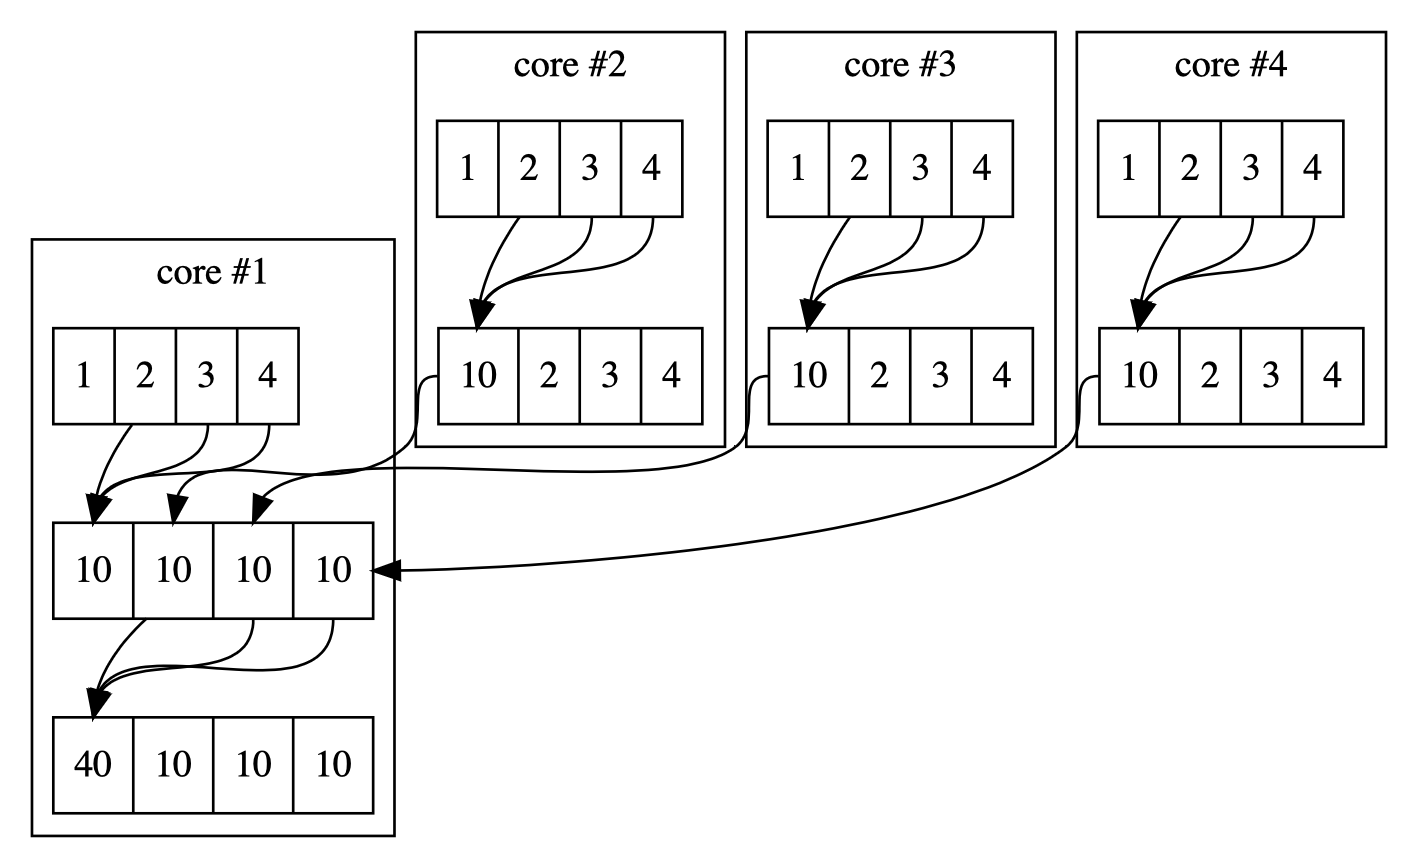
\includegraphics[scale=0.25]{./assets/freduc.png}
  \caption{Visualization of 16-valued vector sum reduction over 4 invocation "cores". The final result is 40, found at index 1 of core \#1, supposing indexing starts from 1.}
  \label{fig:freduc}
\end{figure}

As mentioned previously in this study, the Idris 2 presents the quantification of types. While we did not use Idris 2 in this study, the quantification would be interesting for correctness for parallel computing. Suppose this optimized strategy of making a sum reduction: we have 12 values, and each core can handle four values. Each core has a SIMD width of 4. As such, each core can sum all the values in a single call. To visualize, this operation would look as in Fig. \ref{fig:freduc}. To elaborate, suppose indexing starts from 1. What happens is the following:

\begin{enumerate}
    \item Each core sums its value to the core-local index position 1.
    \item Then, the value is synchronized over shared (i.e., uniform) memory to the "workgroup" leader to a data location that equals the origin core number.
    \item The workgroup leader makes a final sum reduction over the now-synchronized shared values.
    \item The result of the sum reduction operation is found from the index location 1 of the core \#1.
\end{enumerate}

Here, quantification would allow us to reason about the uniqueness of values. For the correctness property, we should ensure that the vector indices of the target vector are unique for each core. Further, no other thread is writing or reading to the critical sections while such values are computed. Given the assumptions of well-typed APL, capturing the modeling is possible statically: the uniqueness would be enforced by quantifying each copy and reducing operations of each core, and correct addressing comes from shape inference via dependent types. In other words, it could be possible to prove that a sum reduction of 16 values is about the operation of 4 multiples of SomeVect 4 disjoint vectors, which involves Reduce + Sync + Reduce operation path, and use the fact that the vectors are disjoint pieces from the initial vector that the target index assigned to them comes from this disjoint property. Thus there can be no indexing errors in the operation as a whole.

Quantifying the operations instead of the values would also make it possible to implement thoughts of the aforementioned dependence logic, but not for values, but functions. It could be interesting for future studies to attempt to reason about properties such that the result can be constructed in $N$ steps using $f$ function. Another aspect could be to compiler optimizations to prove redundancies of some two-phased computation: i.e., an attempt at automatic idiom-capturing, as explained as a common optimization tactic in current-day APL interpreters (see: \cite{hui2020apl}).

\section{Dependently Typed APL}
\label{sc:dependentapl}

In an online available conference meet-up\footnote{\url{https://www.youtube.com/watch?v=x3y22-cMBMQ}}, the main author of Idris addressed the idea of introducing dependent types in small phases to computer science students via a programming language that hides away the typing. It is worth noting that, in a sense, dependently typed APL as presented in this thesis work could fit the niche: on the APL level, the language has no explicit types and abstracts away concepts of iterators and for loops. Then, there is the second layer of the language via typing: the concept of static analysis could be introduced by abstractively interpreting the APL programs for shape errors in Idris. Next, the third level is the actual implementation of the operands in some chosen language.

\section*{Summary}

In the future, it would be interesting to apply Idris 2 to our current version for more comprehensive parallel modeling. Dependent APL could also be considered an exciting avenue for learning purposes, both from the perspective of array programming and dependent types.

\chapter{Conclusion}
\label{ch:conclusion}

%- reflection per the whole thesis project
%- mirror the intro
%- what the thesis was about
%- what went well, what did not, what i would different, future work
%- does it work, repeat
%- what to do if they would continue,

This study was motivated by the need to add a type system for GPU programs. This need was identified in a previous study, in which we had to do it manually. We chose dependently typed Idris to do this. We found that shape analysis done with Idris can help parallel program execution in two ways: a) in scheduling and b) in vectorizing bytecode. Having chosen APL as the modeled parallel language, we found that a type system could be added without any semantic changes to APL itself, thanks to how strict APL is. We demonstrated the ability to detect shape errors, and on the other hand, the ability to parse strongly typed intermediary types for our initial purpose. This is useful for correctness and performance reasons: we know that scheduled programs will not go wrong, and we know precisely the amount of resources our computation tasks use. Future studies could exploit this static information to split computation into smaller pieces. This might be useful in a network of GPUs, in which tasks are broadcasted into a distributed network.

To realize the system and the approach proposed in this study, Idris, and thus functional programming, had to be learned. It seems that without a functional programming paradigm, creating a similar approach is not currently possible. We remark that the notion of recursive data structures does not directly aid in our specific application, as much as pattern matching, theorem proving, and termination checking do. While Idris did not prove to be limited in \emph{what} it can express, challenges were faced in \emph{how} it can express such information. For example, the use of record had to be exploited because it masks the full type signature from function definitions, making the underlying shape data easier to modify. To elaborate:

\begin{verbatim}
f : Shape q (MkDim (S n) (S v)) -> Shape rank (MkDim (S rows) (S stride))
f o = SomeScalar
\end{verbatim}

It gives an error, but with a record returned, it does not:

\begin{verbatim}
record Phase where
  constructor MkPhase
  operation : Operation
  shape : Shape rank (MkDim (S rows) (S stride))
  par : Parallelism x y
...

f : Shape q (MkDim (S n) (S v)) -> Phase
f o = MkPhase Slash SomeScalar (mkPar 0 0)
\end{verbatim}

Even though it seems like the two are equivalent, these challenges would probably be circumvented after more learning to choose the proper functional programming abstractions. However, nevertheless, the initial goal was met regardless. Other challenges included the extensive background of the study: much time was spent on refining the fundamental importance of Idris. Many related works also attempt to capture the data effect done to arrays via the APL functions. However, it soon became evident that an attempt to model actual parallel computation in Idris was fighting the windmills. A resolution was much more abstract than initially planned. While depressing on the code output front, the higher abstraction cut the chase straight into the types, which allowed more thought to be put into classifying programs and parallelism. Yet, the model is easy to extend in future work. Future work would also include approaches to complete mechanization of typing the SPIR-V programs. There is no read-eval-print-loop or foreign-function-interface coded into the program, which would be required when the actual GPU scheduler code via Rust asks for type-checking. At the same time, upgrading to Idris 2 probably makes sense.

Alas, despite general difficulties, the project was finally successful: given an upstream APL parser, it should be trivial to import APL programs from Dyalog APL into Idris, which when run on the GPU, first resolves the typing when parameters are known, then prepares the distribution of the workload evenly on the GPU using the type information, then inserts the types into SPIR-V program source code via specialization constants, and finally runs the program. In effect, It closes the loop for APL to SPIR-V compiler, started a year ago, while also abstracting the use of dependent types in such a way that retains the upsides of static type checking while keeping the APL code the same as before. Though the type checking will not work for nondeterministic APL programs, this is not an issue because GPUs cannot run such programs with excellent performance. Moving forward, it seems worthwhile to study the machine-to-machine distribution of the GPU programs. Because the type checking in Idris is terminating, we know that we can always type them for the operands that we support. When optimizing the distribution of the execution among many computers, this might be relevant property, proving that an optimal distribution always exists. This is generally not the case with TensorFlow and other related work, nor do those projects' computations reside within the strict boundaries set by APL. Researching the duality of semantically strict but implicitly typed programming language, but which under-the-hood is supercharged with dependent types, could be something interesting to trivialize.

\appendix
\chapter{SPIR-V code artifacts}

\begin{figure}

    \begin{lstlisting}[
        basicstyle=\tiny, %or \small or \footnotesize etc.
    ]
; SPIR-V
; Version: 1.3
; Generator: Khronos SPIR-V Tools Assembler; 0
; Bound: 36
; Schema: 0
               OpCapability Shader
          %1 = OpExtInstImport "GLSL.std.450"
               OpMemoryModel Logical GLSL450
               OpEntryPoint GLCompute %main "main" %gl_GlobalInvocationID
               OpExecutionMode %main LocalSize 1 1 1
               OpSource GLSL 450
               OpName %main "main"
               OpName %index "index"
               OpName %gl_GlobalInvocationID "gl_GlobalInvocationID"
               OpName %LeftBuffer "LeftBuffer"
               OpMemberName %LeftBuffer 0 "numbers"
               OpName %lhs "lhs"
               OpName %RightBuffer "RightBuffer"
               OpMemberName %RightBuffer 0 "numbers"
               OpName %rhs "rhs"
               OpDecorate %gl_GlobalInvocationID BuiltIn GlobalInvocationId
               OpDecorate %_runtimearr_float ArrayStride 4
               OpMemberDecorate %LeftBuffer 0 Offset 0
               OpDecorate %LeftBuffer BufferBlock
               OpDecorate %lhs DescriptorSet 0
               OpDecorate %lhs Binding 0
               OpDecorate %_runtimearr_float_0 ArrayStride 4
               OpMemberDecorate %RightBuffer 0 Offset 0
               OpDecorate %RightBuffer BufferBlock
               OpDecorate %rhs DescriptorSet 0
               OpDecorate %rhs Binding 1
       %void = OpTypeVoid
         %12 = OpTypeFunction %void
       %uint = OpTypeInt 32 0
%_ptr_Function_uint = OpTypePointer Function %uint
     %v3uint = OpTypeVector %uint 3
%_ptr_Input_v3uint = OpTypePointer Input %v3uint
%gl_GlobalInvocationID = OpVariable %_ptr_Input_v3uint Input
     %uint_0 = OpConstant %uint 0
%_ptr_Input_uint = OpTypePointer Input %uint
      %float = OpTypeFloat 32
%_runtimearr_float = OpTypeRuntimeArray %float
 %LeftBuffer = OpTypeStruct %_runtimearr_float
%_ptr_Uniform_LeftBuffer = OpTypePointer Uniform %LeftBuffer
        %lhs = OpVariable %_ptr_Uniform_LeftBuffer Uniform
        %int = OpTypeInt 32 1
      %int_0 = OpConstant %int 0
%_runtimearr_float_0 = OpTypeRuntimeArray %float
%RightBuffer = OpTypeStruct %_runtimearr_float_0
%_ptr_Uniform_RightBuffer = OpTypePointer Uniform %RightBuffer
        %rhs = OpVariable %_ptr_Uniform_RightBuffer Uniform
%_ptr_Uniform_float = OpTypePointer Uniform %float
       %main = OpFunction %void None %12
         %25 = OpLabel
      %index = OpVariable %_ptr_Function_uint Function
         %26 = OpAccessChain %_ptr_Input_uint %gl_GlobalInvocationID %uint_0
         %27 = OpLoad %uint %26
               OpStore %index %27
         %28 = OpLoad %uint %index
         %29 = OpLoad %uint %index
         %30 = OpAccessChain %_ptr_Uniform_float %rhs %int_0 %29
         %31 = OpLoad %float %30
         %32 = OpAccessChain %_ptr_Uniform_float %lhs %int_0 %28
         %33 = OpLoad %float %32
         %34 = OpFAdd %float %33 %31
         %35 = OpAccessChain %_ptr_Uniform_float %lhs %int_0 %28
               OpStore %35 %34
               OpReturn
               OpFunctionEnd
    \end{lstlisting}
    \caption{The code snippet in Fig. \ref{fig:kernel} disassembled into SPIR-V.}
    \label{fig:addition}
\end{figure}

{
\renewcommand*{\bibfont}{\small}
\printbibliography
}

\end{document}
